\documentclass{article}

%                      
% NeurIPS 2026 style. The "default" option = "main" = anonymized review.
% For camera-ready, swap to: \usepackage[final]{neurips_2026}
% For arXiv preprint, swap to: \usepackage[preprint]{neurips_2026}
\usepackage{neurips_2026}


% Math
\usepackage{amsfonts}
\usepackage{amsmath}
\usepackage{amssymb}
\usepackage{amsthm}

% Encoding & fonts
\usepackage[utf8]{inputenc}
\usepackage[T1]{fontenc}
\usepackage{nicefrac}
\usepackage{microtype}

% Links & URLs
\usepackage{hyperref}
\usepackage{url}

% Tables
\usepackage{booktabs}
\usepackage{multirow}
\usepackage[table]{xcolor}

% Figures & layout
\usepackage{graphicx}
\usepackage{wrapfig}
\usepackage{float}

% Captions - load ONCE with options
\usepackage[font=footnotesize,labelfont=bf]{caption}

% Algorithms - load algpseudocode ONLY, never algorithmic
\usepackage{algorithm}
\usepackage{algpseudocode}

% Boxes
\usepackage{tcolorbox}
\usepackage{colortbl}

%                      
% Theorem environments (LLNCS provides these by default; NeurIPS does not)
\newtheorem{theorem}{Theorem}
\newtheorem{proposition}[theorem]{Proposition}
\newtheorem{lemma}[theorem]{Lemma}

%                      
% Convenience macros (replace eccvabbrv functionality)
\newcommand{\etal}{\textit{et~al.}}
\newcommand{\eg}{\textit{e.g.}}
\newcommand{\ie}{\textit{i.e.}}
\usepackage{graphicx}   % Required for \includegraphics
\usepackage{wrapfig}    % Required for the wrapfigure environment
\usepackage{amsmath}    % Recommended for math symbols like P(X|Y)
\usepackage{caption}    % Useful for better control over figure captions
\usepackage[font=footnotesize,labelfont=bf]{caption}
%                      
\usepackage{tcolorbox}
\usepackage{colortbl}
\title{Class-Conditional Knowledge-Guided Learning for Resolving the Generalization--Tail Trade-Off via an Agentic Framework}

% Anonymous review: leave \author block empty; the style file handles it.
% For camera-ready (\usepackage[final]{neurips_2026}), fill in:
% \author{%
%   Bin Xu\thanks{Equal contribution.} \\
%   IMPACT Lab, Arizona State University \\
%   \texttt{bxu29@asu.edu} \\
%   \And
%   Author Two \\
%   Affiliation \\
%   \texttt{email@institution.edu} \\
% }
\linespread{0.90}
\begin{document}

\maketitle
\begin{abstract}
Deep learning models deployed in real-world settings must generalize across heterogeneous domains while remaining reliable on rare and underrepresented classes. However, domain generalization and long-tailed recognition are inherently conflicting objectives: domain-invariant learning favors smooth shared representations, whereas rare-class learning requires highly discriminative boundaries. This challenge is particularly critical in clinical applications, where clinically important conditions remain consistently rare across institutions, imaging devices, and patient populations. We propose \textbf{Retrieve--Reason--Run Agents (R3A)}, a knowledge-guided agentic framework that jointly addresses domain shift and long-tailed imbalance through Class-Conditional Knowledge Routing (CCKR). Instead of conventional feature concatenation, CCKR dynamically routes predictions between knowledge-guided and data-driven models using class-conditional decision cascades. R3A employs coordinated agents to retrieve expert knowledge, reason over causal priors, and automatically construct executable learning pipelines.We evaluate R3A across 10 datasets spanning four clinical applications and modalities, including diabetic retinopathy grading, seizure onset zone localization, echocardiographic cardiac-function assessment, and coronary artery disease detection from ECG. Across in-domain, single-domain, and multi-domain generalization settings, R3A consistently improves rare-class recognition and cross-domain robustness, achieving average gains of 14.14\% in-domain, 16.09\% out-of-domain, and 13.1\% rare-class F1 over strong DG and long-tail baselines. In addition, the framework reduces reliance on extensive expert annotations by autonomously constructing clinically informed pipelines.
\end{abstract}
\section{Introduction}
\label{sec:intro}

As observed by Gu \etal~\cite{Gu22}, the inability of deep-learning models to
generalize in real-world settings arises from variability in both the
categorical distribution $P(Y)$ and the class-conditional distribution
$P(X|Y)$. In medical image analysis these shifts are particularly severe:
multi-center MRI or retinal datasets exhibit large domain gaps from differences
in scanner hardware, acquisition parameters, and patient
demographics~\cite{Lei22, Chen23}. Such variations distort $P(X|Y)$ and
degrade reliability in unseen clinical environments.

Two intertwined challenges dominate this generalization failure:
\textbf{Domain Generalization (DG)} and \textbf{Long-Tailed Visual Recognition
(LT-VR)}. DG aims to learn domain-invariant features stable across
environments~\cite{Wang21}, while LT-VR demands discriminative modeling of
rare disease categories from a highly skewed $P(Y)$~\cite{Zhang21, Li18}. In
clinical data a few prevalent (head) conditions dominate, while rare and
often critical (tail) pathologies are sparsely represented~\cite{CXR24}.
Models trained on such data overfit head classes and catastrophically
misclassify tail diseases.

Although DG and LT-VR have been extensively studied in isolation, they coexist in real-world medical settings. Existing DG methods typically report improvements in macro-level accuracy and cross-domain performance; however, they often fail to preserve performance on rare classes under domain shift, as demonstrated in Table\ref{tab:perclass_f1}. For example, in diabetic retinopathy (DR) grading, which involves five classes where the fourth class (Proliferative DR) is rare, training a Vision Transformer (ViT)-based state-of-the-art empirical risk minimization (ERM) model on the APTOS dataset and evaluating on a different domain, such as MESSIDOR, leads to a drop in overall accuracy. While introducing a DG-enhanced ViT variant \cite{Galappaththige2024} improves in-domain and cross-domain macro performance, the accuracy on the rare class degrades in both settings, despite using the same underlying architecture. Such behavior is unacceptable in high-stakes applications such as autonomous driving, clinical diagnosis, and drone perception, where improvements must be consistent across both frequent and rare classes. (The detailed experimental setup is provided in the appendix 

\ref{table1}.)
\begin{wraptable}{r}{0.575\textwidth}
\centering
\vspace{-0.1in}
\scriptsize

\setlength{\tabcolsep}{2pt}
\renewcommand{\arraystretch}{0.9}

\caption{%
  Comparision of VITERM, VITSPSD and OUR METhod on Per-class F1 (\%) of Train on Aptos and test on APTOS
  (in-domain held-out test set, $n=733$)
  and Messidor (cross-domain, $n=1744$).
  \colorbox{red!20}{\strut~G4 PDR~}~=
  clinically critical rare class
}

\label{tab:perclass_f1}

\resizebox{\linewidth}{!}{%
\begin{tabular}{l cc ccc}
\toprule
\multirow{2}{*}{\textbf{Class}}
  & \multicolumn{2}{c}{%
    \textbf{APTOS (in-domain)}}
  & \multicolumn{3}{c}{%
    \textbf{Messidor (cross-domain)}} \\
\cmidrule(lr){2-3}
\cmidrule(lr){4-6}
  & ERM\_ViT
  & ERM\_SPSD
  & ERM\_ViT
  & ERM\_SPSD
  & \textbf{Ours} \\
\midrule
G0 Normal
  & $93.9 \pm 0.4$
  & $\mathbf{95.0 \pm 0.3}$
  & $21.6 \pm 0.8$
  & $28.5 \pm 0.6$
  & $\mathbf{76.5 \pm 0.5}$ \\
G1 Mild
  & $47.9 \pm 1.1$
  & $\mathbf{54.8 \pm 0.9}$
  & $0.0 \pm 0.0$
  & $0.0 \pm 0.0$
  & $\mathbf{4.8 \pm 0.4}$ \\
G2 Moderate
  & $67.6 \pm 0.7$
  & $\mathbf{70.2 \pm 0.5}$
  & $24.7 \pm 0.9$
  & $30.3 \pm 0.7$
  & $\mathbf{29.1 \pm 0.6}$ \\
G3 Severe
  & $16.0 \pm 1.2$
  & $\mathbf{20.0 \pm 1.0}$
  & $1.3 \pm 0.5$
  & $5.9 \pm 0.8$
  & $\mathbf{29.3 \pm 0.7}$ \\
\rowcolor{red!20}
\textbf{G4 PDR}
  & $\mathbf{11.8 \pm 1.3}$
  & $6.6 \pm 1.1$
  & $8.6 \pm 1.1$
  & $3.3 \pm 0.9$
  & $\mathbf{18.5 \pm 0.8}$ \\
\midrule
\rowcolor{red!20}
\textbf{macro-F1}
  & $47.4 \pm 0.6$
  & $\mathbf{49.3 \pm 0.5}$
  & $11.2 \pm 0.4$
  & $13.6 \pm 0.3$
  & $\mathbf{31.6 \pm 0.4}$ \\
\bottomrule
\end{tabular}%
}

\vspace{-0.15in}
\end{wraptable}
Recent work on \textbf{Multi-Domain Long-Tailed (MDLT) Recognition}~\cite{Yang22} attempts to jointly address DG and LT-VR; however, it assumes that long-tailed distributions exist in some domains but not others, allowing the model to implicitly learn tail classes across multiple domains. This assumption does not hold in real-world scenarios, where rare classes remain consistently rare across all domains. For instance, proliferative diabetic retinopathy and pancreatic cancer remain rare irrespective of the dataset or clinical setting. Within this joint DG and LT-VR setting, a fundamental optimization
conflict therefore emerges: DG objectives favor \emph{broad, smooth minima}
that promote domain invariance~\cite{Su24, Su24a}, while LT-VR objectives
enforce \emph{sharp, discriminative minima} for minority-class
separation~\cite{TSCNet25}. Jointly optimizing the two produces destructive
gradient interference that degrades both generalization and tail-class
performance~\cite{Yang22, Zhang21, Su24a}.

Conventional DG methods assume $P(Y|X)$ is invariant across
domains~\cite{li2018domain}. This rarely holds in medicine, where both $P(X)$
and $P(Y|X)$ vary. The diagnostic definition of coronary artery disease
(CAD) from invasive coronary angiography, for instance, ranges from $>50\%$
to $>70\%$ stenosis across institutions~\cite{vazquez2024clinical}.
Consequently, exercise-stress ECG studies labeled "true positive" reflect
different criteria, inducing shifts in both $P(Y|X)$ and $P(Y)$. State-of-the-art
DG methods that rely solely on data-driven feature invariance therefore cannot
generalize across domains with such label-generation variability unless they
explicitly incorporate clinical knowledge.

When the conditional and prior distributions both shift, generalization can be
improved by integrating \textbf{domain-invariant knowledge} $K$. Several
application-specific works concatenate clinical knowledge with data-driven
features~\cite{Wong22, Hohn21_Cancer, Gessert20, Tschandl23, Hohn21_JMIR}.
A common augmented representation is $h'(X) = [h(X), K]$, yielding
\[
P(h'(X), Y) = P(h(X)|Y)\, P(K|Y)\, P(Y),
\]
where $P(K|Y)$ encodes invariant causal clinical relationships. However, such
representations rely on a domain-invariant data-driven $P(h(X)|Y)$ that is
independent of knowledge, which is not guaranteed for rare classes given
training imbalance. If $P(h(X)|Y)$ is poor, then even with strong $P(K|Y)$ the
multiplicative combination is inconclusive. Many works that incorporate
clinician knowledge into deep-learning pipelines therefore find concatenation
unhelpful~\cite{Wong22, Hohn21_Cancer, Gessert20, Tschandl23, Hohn21_JMIR}.
Recent work shows that \emph{class-conditional} integration if-then-else
combination of deep learning and clinical knowledge is more effective for
rare-class discrimination than concatenation~\cite{Hohn21_Cancer,
banerjee2023automated, kamboj2024expert, kamboj2024expertTAI}.


\textbf{Contributions.} We formalize and prove that class-conditional
Class-Conditional Knowledge Routing (CCKR) has a higher likelihood of achieving better
performance than concatenation in long-tailed domain generalization settings using knowledge-based expert machines.
Building on this theory we propose the \textbf{Retrieve–Reason–Run Agent
(R3A)} framework, which builds knowledge-guided deep-learning decision trees
to jointly resolve domain and long-tail challenges. R3A automatically
retrieves, structures, and integrates clinically validated knowledge and
demographic priors from biomedical literature into a causal knowledge base.
Through an agentic, reinforcement-driven pipeline, R3A iteratively refines
feature detectors and aligns learned representations with domain-invariant
causal cues. Experiments on 10 medical-imaging datasets across four
modalities show that R3A consistently outperforms state-of-the-art DG and
LT-VR baselines and reduces manual annotation burden.

\section{Related Work}
\label{sec:relWorks}

\textbf{Long-Tailed Category Distribution.}
Classical approaches rebalance training signals through data-level
resampling~\cite{Han05, Buda18}, class-level
reweighting~\cite{Huang16, Wang17}, or output-level calibration such as
logits adjustment and balanced meta-softmax~\cite{Hong21, Ren20}. Two-stage
strategies~\cite{Kang19, Tang20} decouple representation learning from
classifier optimization. Newer work uses ensemble and contrastive
paradigms~\cite{Wang21contrast}, knowledge distillation~\cite{Iscen21}, and
expert routing~\cite{Wang21routing}. Most assume identical conditional
distributions across classes and domains, overlooking the interaction between
imbalance and domain shift common in medical imaging.

\textbf{Domain Generalization (DG).}
DG strategies include conditional invariant representation
learning~\cite{Li18}, domain disentanglement~\cite{Wang20disentangle, Gu20},
and episodic meta-learning~\cite{Li19}. Others augment training diversity via
domain simulation or style mixing~\cite{Dou19, Mancini20, Zhou21}. Most assume
balanced classes, which limits performance under
\emph{long-tailed domain shifts (LT-DS)}.

\textbf{Multi-Domain and Long-Tailed Recognition (MDLT).}
Recent work unifies long-tailed recognition and domain generalization under the MDLT paradigm~\cite{Yang22}. Methods such as BoDA~\cite{Yang22}, TALLY~\cite{Yao22}, and FedTAIL~\cite{Su24} primarily address \emph{multi-source} settings, where domain--class priors vary across sources and tail classes in one domain can be partially compensated by head examples from other domains~\cite{CXR24, Shu21}. In contrast, our work considers a more realistic setting in which rare classes remain rare across all domains, i.e., $\mathbb{P}(Y = y_{\text{tail}})$ remains consistently low for all domains $d \in \mathcal{D}$. We further study a domain generalization scenario where training may be restricted to a single source domain, and the tail-class prevalence in the target domain is either stable or distributionally shifted, making cross-domain compensation for rare classes fundamentally infeasible in practice.

\textbf{Relation to classical decision fusion.}
While classical sum- and product-rule decision fusion schemes have been theoretically analyzed (\eg, Kittler \etal~\cite{kittler1998}), these approaches operate at the level of unconditional posterior aggregation, i.e., $P(y \mid x) \propto \sum_i P_i(y \mid x)$ or $\prod_i P_i(y \mid x)$. In contrast, our formulation specializes fusion into a \emph{class-conditional, knowledge-guided routing/cascade} mechanism, where decisions are conditioned on structured priors and intermediate expert selection. A detailed comparison with ensemble learning and mixture-of-experts formulations is provided in Section~\ref{app:kittler_moe}.

\begin{wrapfigure}{r}{0.35\textwidth} % Narrowed the wrap area
    \centering
    \vspace{-15pt} 
    % Image scaled down to fit the narrower wrapfigure
    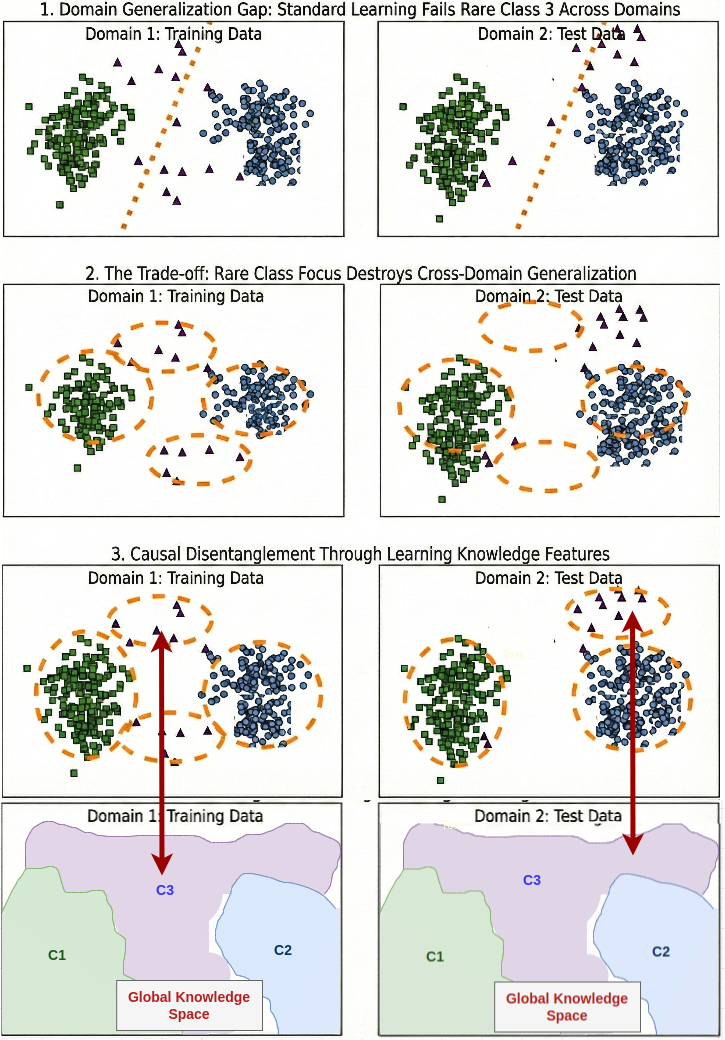
\includegraphics[trim=0 0 0 0, clip, width=0.95\linewidth]{problemFormulation.png} 
    
    % \footnotesize makes the caption text significantly smaller
    \caption{\footnotesize \textbf{The Domain Generalization vs Long-Tailed Trade-off.} 
    (1) Standard learning fails on C3. 
    (2) $P(X_d \mid Y)$ captures unstable correlations. 
    (3) Domain-invariant space recovers C3 globally.}
    \label{fig:problemFormulation}
    \vspace{-10pt}
\end{wrapfigure}
    \vspace{-14pt}
\section{Formalization of DG Solutions}
\label{sec:formal}
\subsection{Problem Setting}
\label{sec:problem}
Figure~\ref{fig:problemFormulation} illustrates the trade-off between
generalization and rare-class fidelity under domain shift.
\textbf{(1)}~Optimizing for dominant causal signals stable in $P(X_d)$
fails to separate rare-class representations ($p(Y=r) \ll 1$), collapsing
their manifolds across domains.
\textbf{(2)}~Fitting finer-grained $P(X_d \mid Y)$ captures non-causal,
domain-dependent correlations that fail when $P(X_1 \mid Y) \neq P(X_2 \mid Y)$.
\textbf{(3)}~We resolve this via a \emph{domain-invariant knowledge space}
$K$, where $P(K \mid Y)$ encodes globally valid causal semantics. Anchoring
representations in $K$ disentangles causal from non-causal factors,
jointly enabling (i) a visual causal feature space for cross-domain
generalization and (ii) a knowledge feature space for class-specific
fidelity, including rare conditions.

This dual-space paradigm is realized by the proposed \textbf{CCKR
algorithm} (Alg.~\ref{alg:CCKR}, Fig.~\ref{fig:medxai_framework}), which
integrates visual features from raw data with knowledge features from
structured priors. CCKR builds a class-conditional classifier guided by
\textbf{Entropy Imbalance Gain (EIG)} and a \textbf{purity index} for
tree-based partitioning over both spaces. Empirically, CCKR outperforms
state-of-the-art baselines on in-domain, single-domain, and multi-domain
generalization, improving rare-class prediction while maintaining overall
accuracy.

\subsection{Drawbacks of Existing DG Solutions}
The intuitive solution seeks $h \in \mathcal{H}$ minimizing the expected
target risk under unseen target distributions $P_T \neq P_S$.
\begin{equation}
\mathcal{R}_T(h) = \mathop{\mathbb{E}}\limits_{(\mathbf{x},y)\sim P_T}[\ell(h(\mathbf{x}),y)],
\end{equation}


\paragraph{Theoretical bound of DG risk.}
Following Ben-David~\etal~\cite{BenDavid10} and its class-conditional
extension~\cite{Yang22}, the per-class generalization bound under domain
shift is
\begin{equation}
\label{eq:classrisk}
\mathcal{R}_{T,c}(h) \le \widehat{\mathcal{R}}_{S_c}(h)
+ \underbrace{\tfrac{1}{2}d_{\mathcal{H}\Delta\mathcal{H}}(S_c, T_c)}_{\text{domain divergence}}
+ 2\mathfrak{R}_{n_c}(\mathcal{L}\circ\mathcal{H})
+ \underbrace{\sqrt{\tfrac{\log(2/\delta)}{2 n_c}}}_{\text{class rarity}}
+ \lambda_c,
\end{equation}
where $d_{\mathcal{H}\Delta\mathcal{H}}$ is the empirical domain
discrepancy, $\mathfrak{R}_{n_c}$ the Rademacher complexity, and
$\lambda_c$ the Bayes approximation error. The bound has two key
dependencies: (i) the class-sample size $n_c$, which tightens for frequent
classes but loosens for rare ones, and (ii) the domain divergence
$d_{\mathcal{H}\Delta\mathcal{H}}(S_c, T_c)$, which inflates as
class-conditional covariate shifts increase. Tail classes with small $n_c$
and high domain discrepancy thus see the largest risk
amplification~\cite{Yang22, Zhang21}.

\paragraph{Conflict between DG and rare-class objectives.}
DG and LT-VR objectives push the model toward distinct loss-landscape regimes.
DG regularization seeks \emph{flat minima} for domain robustness, minimizing
the loss-Hessian spectral norm
\begin{equation}
\mathcal{R}_{DG} = \mathbb{E}_{\mathbf{x}}\|\nabla^2_{\theta}\ell(h_{\theta}(\mathbf{x}))\|_2^2,
\end{equation}
while long-tail (LT) weighting magnifies rare-class gradients, emphasizing
\emph{sharp minima}
\begin{equation}
\mathcal{R}_{LT} = \sum_{c=1}^K w_c\, \mathbb{E}_{(\mathbf{x},y)\in S_c}\ell(h_{\theta}(\mathbf{x}), y),
\end{equation}
with $w_c \propto n_c^{-\gamma}$ and $\gamma > 0$~\cite{Cui19}. The
resulting gradient misalignment between $\nabla_{\theta}\mathcal{R}_{DG}$
and $\nabla_{\theta}\mathcal{R}_{LT}$ produces unstable
convergence~\cite{Su24}. This smoothness--sharpness conflict has been
observed empirically across multi-domain
benchmarks~\cite{Yang22, Su24a, Tang25, FRoundation25}.



\begin{figure}[t]
    \centering
    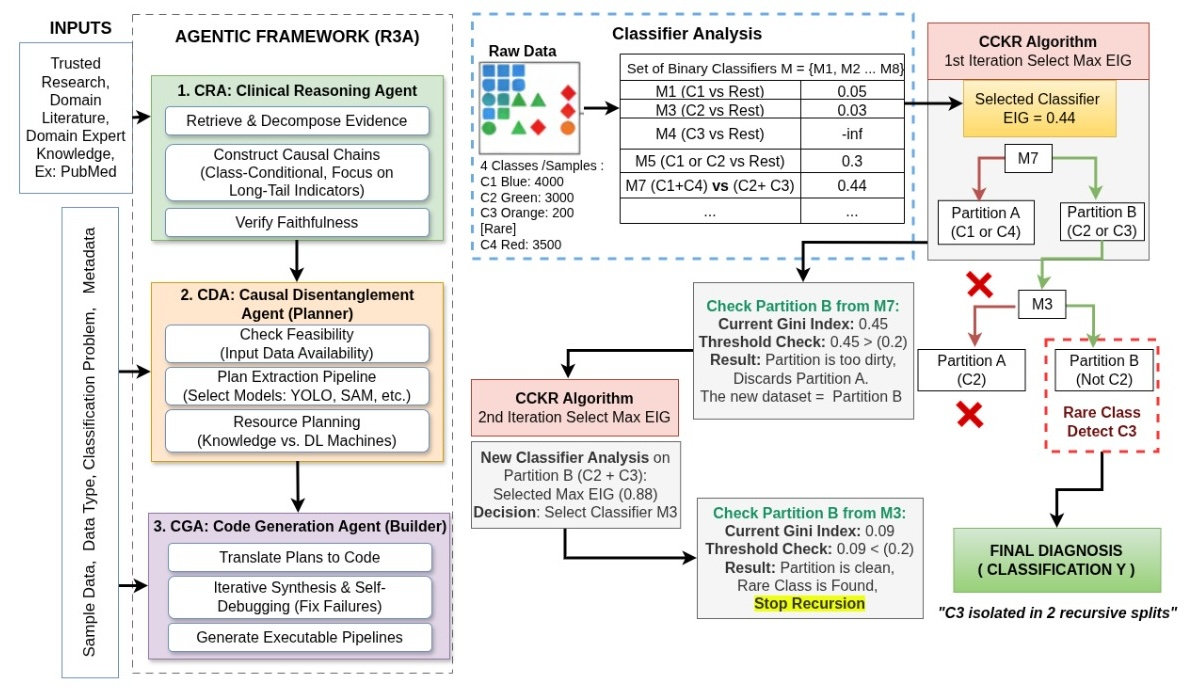
\includegraphics[width=0.99\linewidth]{final-pipeline-1.jpg}
    \caption{\textbf{Overview of the Retrieve–Reason–Run Agent (R3A)
    Framework with Class-Conditional Knowledge Routing (CCKR).}
    Three coordinated agents: (1) a Clinical Reasoning Agent retrieves
    evidence and constructs class-conditional causal chains; (2) a Causal
    Disentanglement Agent plans feature extraction and model selection under
    data and resource constraints; (3) a Code Generation Agent implements
    executable pipelines. The CCKR algorithm iteratively selects classifiers
    using entropy imbalance gain (EIG) to isolate rare classes via
    recursive partitioning.}
    \label{medxai_framework2}
\end{figure}

\section{Class-Conditional Knowledge Routing}
\label{sec:CCKR}

Assume a hypothesis set $H(X) = \{h_1(X), \ldots, h_m(X)\}$, where some
$h_i$ are data-driven (\eg, deep learning models) and others are
knowledge-driven (\eg, clinical rules). Let $h_i(x)$ for $i \le m_k$ be
knowledge-driven, and the remainder data-driven. For each class
$y_j \in \mathcal{Y}$, let $\phi_{y_j}$ be an if-then-else rule combining
$H(X)$ to obtain a class-specific hypothesis. The combinator can be learned
as a path in a decision tree as shown in Figure \ref{medxai_framework2}:
\begin{itemize}
\item \textbf{Step 1:} apply a hypothesis from $H(X)$,
\item \textbf{Step 2:} decide if it predicts class $y_j$,
\item \textbf{Step 3:} evaluate purity of the decision,
\item \textbf{Step 4:} if purity exceeds a threshold, terminate the branch,
\item \textbf{Step 5:} otherwise continue with a new $h(X)$ and repeat Step~1,
\item \textbf{Stopping condition:} the tree stops at a class-specific depth
$b_j$.
\end{itemize}

Let $h_{i_t}$ be the hypothesis applied at depth $t$ of the conditional
branch. Define the admission function for class $y_j$ at step $t$ as
\[
\alpha_{j,t}(x) = \mathbb{I}\!\left(h_{i_t}(x) = y_j\right),
\]
where $\mathbb{I}(\cdot)$ is an indicator. Let
$\pi_{j,t}(x) \in [0,1]$ denote a purity/confidence score of $h_{i_t}$ for
$y_j$, and let $\theta_j$ be a class-specific threshold. The
\emph{first-conclusive-step gate} is
\begin{equation}
\psi_{j,t}(x) = \mathbb{I}\!\left(\alpha_{j,t}(x)=1 \;\wedge\; \pi_{j,t}(x) \ge \theta_j\right)
\cdot \prod_{s=1}^{t-1} \mathbb{I}\!\left(\pi_{j,s}(x) < \theta_j\right).
\end{equation}

\textbf{Rationale.} In the previous $t-1$ steps the purity threshold was not
met, but at step $t$ we achieve conclusive confidence for $y_j$. The final
class-specific hypothesis is
\begin{equation}
\label{eqn:CCKR}
\phi_{y_j}(x) = \sum_{t=1}^{b_j} \psi_{j,t}(x)\, h_{i_t}(x).
\end{equation}
By construction at most one $\psi_{j,t}(x)$ is $1$ for fixed $(j, x)$, so
\eqref{eqn:CCKR} acts as a path-selector. If $i_t \le m_k$ at step $t$ then
$h_{i_t}$ is a knowledge-driven classifier; otherwise it is data-driven.


\noindent\textbf{Theorem 1.}
CCKR enables disentanglement of domain generalization and long-tail components of the per-class generalization bound.

% =========================
% Theorem 2 (MIN-CHANGE FIX)
% =========================

\noindent\textbf{Theorem 2.}
CCKR approach has a higher likelihood of achieving higher joint probability distribution
$P_T(\phi_{\mathcal{Y}}(X),Y)$ than knowledge concatenation $P_T([h(X),K],Y)$ in the target domain

(\emph{proof are in appendices ~\ref{proof}}).
\subsection{Instance of CCKR}
\label{sec:CCKR_instance}
\begin{wrapfigure}{R}{0.5\textwidth} % Narrowed to 0.5 for better text wrap
\vspace{-32pt} 
\begin{minipage}{0.5\textwidth}

\begin{algorithm}[H] % CRITICAL: Use [H] to prevent the algorithm from floating out of the wrapfigure

\small
\caption{Class-Conditional Knowledge Routing (CCKR)}
\label{alg:CCKR}
\begin{algorithmic}[1]
\Require Data $(x, y)$, rare label $y_r$, thresholds $\tau_m$, $\tau_g$, $d_{th}$, hypothesis set $\mathcal{H}$
\State Initialize active set $\Omega \leftarrow \{(x, y)\}$
\While{$\Omega$ refines meaningfully}
    \State Compute $\mathrm{EIG}(h; \Omega)$ for each $h \in \mathcal{H}$
    \State Let $h_{(1)}, h_{(2)}$ be top-2 by EIG
    \If{$\mathrm{EIG}(h_{(1)}) - \mathrm{EIG}(h_{(2)}) \le \tau_m$}
        \State $\mathcal{T} \leftarrow \{h \mid \text{tied within } \tau_m\}$
        \State $\hat{h} \leftarrow \arg\max_{h \in \mathcal{T}} \mathrm{Dep}(h; \Omega)$
        \State $h^* \leftarrow (\mathrm{Dep}(\hat{h}) \ge d_{th}) ? \hat{h} : h_{(1)}$
    \Else
        \State $h^* \leftarrow h_{(1)}$
    \EndIf
    \State Partition $\Omega$ by $h^* \rightarrow \{ \Omega^{(k)} \}_{k=1}^K$
    \State $s \leftarrow$ rare-enriched branch
    \If{$\mathrm{Gini}(s) > \tau_g$}
        \State $\Omega \leftarrow s$
    \Else \ \textbf{break}
    \EndIf
\EndWhile
\end{algorithmic}
\end{algorithm}
\end{minipage}
\vspace{-35 pt}
\end{wrapfigure}        

Algorithm~\ref{alg:CCKR} provides a practical instantiation of the CCKR framework.
The goal is to dynamically select and cascade hypothesis functions  either
knowledge-driven $h_{\text{kl}}(x)$ or deep learning-driven $h_{\text{dl}}(x)$  so that per-class predictions
are optimized under long-tailed and domain-shift conditions.

\paragraph{Setup.}
Given paired samples $(x,y)$ and a target rare label $y_r$, we initialize an active set
$\Omega \subseteq \{(x,y)\}$ (initially, the full dataset or the current node's subset).
Each hypothesis $h\in\mathcal{H}$ induces a partition of $\Omega$ into branches (subsets)
$S_h(\Omega)=\{\Omega^{(1)},\ldots,\Omega^{(K)}\}$, where membership is determined by the discrete outcome of $h$
(e.g., predicted label or binary decision). We cascade only along a single branch that is most relevant to $y_r$.

\paragraph{Entropy Imbalance Gain (EIG).}
We define EIG as the \emph{reduction} in a tail-aware entropy-imbalance statistic.
Let $\mathcal{Y}$ denote the label set and let $p_{\Omega}(y)=\frac{1}{|\Omega|}\sum_{(x,y')\in\Omega}\mathbb{I}[y'=y]$
be the empirical label distribution on $\Omega$.
Define the \emph{tail-weighted entropy per class} as
\begin{equation}
\begin{aligned}
\theta_{\Omega}(y)
&= -\,w(y)\,p_{\Omega}(y)\,\log\!\big(p_{\Omega}(y)+\epsilon\big), \\
w(y)
&= \frac{1}{\big(p_{\Omega}(y)+\epsilon\big)^{\gamma}}.
\end{aligned}
\end{equation}

where $\gamma\ge 0$ emphasizes rare classes and $\epsilon>0$ avoids numerical issues.
Let the \emph{entropy-imbalance deviation} be
\begin{equation}
\eta(\Omega)
\;=\;
\max_{y\in\mathcal{Y}}\theta_{\Omega}(y)\;-\;\frac{1}{|\mathcal{Y}|}\sum_{y\in\mathcal{Y}}\theta_{\Omega}(y).
\end{equation}
For a hypothesis $h$ producing a partition $S_h(\Omega)=\{\Omega^{(k)}\}_{k=1}^{K}$, define the post-split deviation as the
branch-size-weighted average
\begin{equation}
\eta_h(\Omega)
\;=\;
\sum_{k=1}^{K}\frac{|\Omega^{(k)}|}{|\Omega|}\,\eta\!\big(\Omega^{(k)}\big).
\end{equation}
We then define the \textbf{Entropy Imbalance Gain} as
\begin{equation}
\mathrm{EIG}(h;\Omega)
\;=\;
\eta(\Omega)\;-\;\eta_h(\Omega).
\label{eq:eig_def_B}
\end{equation}
Intuitively, $\eta(\Omega)$ captures the \emph{worst-class} tail-weighted entropy deviation on the node,
and $\mathrm{EIG}(h;\Omega)$ measures how much a split reduces this worst-class deviation. This favors hypotheses
that improve tail uncertainty rather than optimizing only head-dominated average entropy.

\paragraph{Rare-branch selection and purity.}
Given the selected $h^*$, we choose the branch $s$ to recurse on as the branch that is most enriched in $y_r$:
\begin{equation}
s \;=\; \arg\max_{\Omega^{(k)}\in S_{h^*}(\Omega)} \frac{1}{|\Omega^{(k)}|}\sum_{(x,y)\in\Omega^{(k)}}\mathbb{I}[y=y_r].
\end{equation}
We quantify purity of the selected branch using Gini impurity
$\mathrm{Gini}(s)=1-\sum_{y\in\mathcal{Y}}p_s(y)^2$ with $p_s(y)$ estimated empirically.
Since Gini is an \emph{impurity} measure, smaller values indicate higher purity; we stop when $\mathrm{Gini}(s)\le \tau_g$ as illustrated in Fig.~\ref{fig:medxai_framework}.

\paragraph{Tie-breaking and stopping.}
Let $\mathrm{EIG}_{(1)}\ge \mathrm{EIG}_{(2)}$ be the best and second-best gains on $\Omega$.
We declare a tie if $\mathrm{EIG}_{(1)}-\mathrm{EIG}_{(2)}\le \tau_m$.
In ties, we use a validation-calibrated \emph{dependability} score on the rare label:
\begin{equation}
\mathrm{Dep}(h;\Omega)
\;=\;
\frac{1}{|\Omega|}\sum_{(x,y)\in\Omega} p_h(y_r\mid x),
\end{equation}
and choose the tied hypothesis with the largest $\mathrm{Dep}(h;\Omega)$, requiring it to exceed $d_{th}$; otherwise we fall back to
the maximum-EIG hypothesis.
To prevent over-deep cascades, we early-stop when $|s|$ is below a minimum node size or when EIG improvements fall below $\delta$
for two consecutive iterations.
CCKR focuses capacity on tail classes while enabling separation between knowledge-driven and data-driven components.
EIG is favored over traditional information gain because it explicitly measures reduction in worst-class tail-weighted entropy deviation
(Eq.~\eqref{eq:eig_def_B}), prioritizing rare-class uncertainty reduction. The Gini index complements this by providing a stable and interpretable
impurity measure for deciding whether further cascading is necessary. To justify the design choice, we include ablations that replace EIG with (i) standard information gain (entropy reduction) and (ii) held-out cross-entropy improvement as split criteria, while keeping the CCKR pipeline fixed (Appendix~\ref{app:eig_baselines}).

\paragraph{Sensitivity analysis.}
We report sensitivity to $\tau_m,\tau_g,d_{th}$ by sweeping one parameter at a time on the validation split:
$\tau_m\in\{0,0.01,0.02,0.05\}$, $\tau_g\in\{0.05,0.10,0.20,0.30\}$, and $d_{th}\in\{0.50,0.60,0.70,0.80\}$,
measuring tail-F1/balanced accuracy, average cascade depth, and tie frequency. Hyperparameters are selected on validation only.
\subsection{Knowledge Extraction for Enabling CCKR}

A central challenge in realizing CCKR is extracting expert knowledge to
guide model decisions. Such extraction often relies on domain experts,
medical annotators, or specialized deep-learning pipelines. Lesion- or
structure-specific cues frequently require fine-tuned object detectors such
as YOLO~\cite{redmon2016yolo}, SAM~\cite{kirillov2023sam}, or
Detectron2~\cite{wu2019detectron2}, or U-Net~\cite{ronneberger2015unet} for
vessel segmentation, each typically trained on $\ge 500$ annotated images
per attribute. This dependence on fine-grained annotations limits CCKR's
scalability. We address this by developing the R3A framework, which autonomously constructs these
pipelines, retrieves domain-specific cues, and organizes them into
structured priors for CCKR, reducing manual involvement.

\section{Proposed Method: Retrieve–Reason–Run Agentic Framework (R3A)}
\label{sec:method}

R3A is a modular agentic pipeline that unifies expert medical knowledge
with deep-neural learning to address domain shift and long-tailed imbalance
in clinical imaging. It uses LLM-driven agents to autonomously retrieve,
structure, and operationalize clinical knowledge, while the downstream CCKR
module adaptively integrates knowledge-trained classifiers $h_K(x)$ with
deep models $h_D(x)$ that learn visual representations. The workflow is
illustrated in Figure~\ref{fig:medxai_framework}. Three core agents
instantiate the pipeline: the \textbf{Clinical Reasoning Agent (CRA)}, the
\textbf{Causal Disentanglement Agent (CDA)}, and the \textbf{Code Generation
Agent (CGA)}.

\subsection{Agentic Knowledge Acquisition and Rule Encoding}

We now detail the first stages of R3A: acquiring symbolic knowledge,
encoding it into features and rules, and preparing it for use in CCKR
hypotheses $h_K(x)$ as illustrated in Figure~\ref{medxai_framework2}.

\textbf{Agent~1 (CRA): Medical Knowledge Retrieval.}
A PubMed-based Retrieval-Augmented Generation system extracts diagnostic
criteria, lesion patterns, imaging biomarkers, and evidence-based decision
rules. For diabetic retinopathy, knowledge for each of the five DR stages
maps into a candidate knowledge feature set
\[
\mathcal{K} = \{k_1, k_2, \dots, k_n\},
\]
where each $k_i$ corresponds to a measurable attribute such as
``hemorrhage present'' or ``gray-matter activation.'' The agent filters
$\mathcal{K}$ to retain only features that can be reliably computed from
available data.

\textbf{CRA: Rule Refinement.}
Textual diagnostic criteria for the retained features $\mathcal{K}$ are
converted into executable symbolic rules. This step adapts the knowledge to
imaging and dataset constraints by defining (1) threshold ranges,
(2) confidence levels, and (3) failure-case handling for conditions such
as optic-disc overlap, low contrast, or motion blur. The resulting rule set
\[
\mathcal{R} = \{r_1, r_2, \dots, r_m\}
\]
specifies how features in $\mathcal{K}$ should be computed and interpreted.
$\mathcal{R}$ is finalized based on input quality, robustness of feature
extraction, and computational resources.

\textbf{Agent~2 (CDA): Architecture Selection.}
Given the target modality and disease, the LLM scans recent publications
and GitHub repositories to identify suitable open-source models. It
proposes modality-specific architectures (\eg, ViT, CNN, transformer
backbones), retrieves pretrained weights, and returns a recommended
configuration. When a backbone is user-specified, the agent reuses it. The
agent also selects $h_K(x)$ classifiers based on $\mathcal{R}$, weighting
code availability, reported performance, computational cost, and
suitability.

\textbf{Agent~3 (CGA): Code Generation.}
For each refined rule $r_i \in \mathcal{R}$, the agent synthesizes Python
programs using OpenCV, PyTorch, and standard detection/segmentation
libraries (YOLO, SAM, Detectron, U-Net, etc.) to produce a set of
extraction routines $\mathcal{C} = \{c_1, c_2, \dots, c_p\}$ each computing a subset of $\mathcal{K}$. Automated input checks, unit
tests, and fallback operations are injected. When a program fails, a
reinforcement-driven refinement loop re-prompts the LLM until correctness
constraints are met. The agent does not blindly trust LLM-produced rules:
it iteratively proposes candidate pipelines and retains only those yielding
measurable gain over the deep-learning-only baseline, discarding
non-improving candidates. The final CCKR cascade therefore uses only
validated knowledge branches and otherwise defaults to deep experts; this
is demonstrated in the ablation of Section~\ref{ablation_study1}.
\vspace{-1.5 pt}
\section{Experiments}
We evaluate R3A across four clinically critical applications spanning neuroimaging, ophthalmology, cardiology, and electrophysiology. For each application, we select benchmark datasets exhibiting long-tailed class distributions with clinically rare but critical categories (details in Table~\ref{table3}). These settings are intentionally chosen to stress-test rare-class recognition under real-world imbalance and distribution shift.  Across all tasks, inputs are inherently multimodal, and R3A demonstrates consistent adaptability to heterogeneous data modalities, datasets, and application-specific constraints. The framework autonomously constructs and refines pipelines by integrating prior literature, task-specific knowledge, and tool-augmented reasoning, enabling robust performance under both domain generalization and out-of-domain generalization settings. Cross-application ID and OOD performance gains are reported in Table~\ref{tab:cross_app_summary}.


\subsection{Application 1: Diabetic Retinopathy Grading}

We evaluate on 5-class DR grading across APTOS, EyePACS, Messidor-1, and
Messidor-2. The hypothesis pool contains ten binary classifiers: five
ViT-based deep models $h_D(x)$ (one per grade) and five knowledge-driven
classifiers $h_K(x)$ from lesion and vessel-morphology rules described in table \ref{app:dr_knowledge}. The CDA
encodes clinical priors (microaneurysm burden, hemorrhage severity, vessel
tortuosity); the CGA uses YOLOv11-based detectors and vessel-analysis
routines to instantiate them; CCKR organizes $h_D(x)$ and $h_K(x)$ into a
knowledge-guided cascade. \paragraph{Results.}
Table~\ref{tab:dr_all_results} summarizes three regimes: (1) \textbf{Normal
DG}, train on APTOS and test on external datasets; (2) \textbf{Single-Domain
Generalization (SDG)}, train on one source and evaluate on unseen targets;
(3) \textbf{Multi-Domain Generalization (MDG)}, leave-one-domain-out
(train on three, test on one). Across settings, R3A/CCKR consistently
improves cross-domain accuracy over the ViT-only branch and DG baselines
(Fishr, SPSD-ViT), with $+5$--$6$ point F1 gains for the rare severe DR stages. The knowledge routed pipeline built by R3A is shown in Figure \ref{fig:dr_framework}.


\begin{table*}[h] % table* spans two columns if using a two-column template
\centering
\scriptsize
\setlength{\tabcolsep}{5pt}
\renewcommand{\arraystretch}{1.2} % Adds a "delicate" vertical breathing room

\caption{\footnotesize \textbf{Generalization Performance across Multi-Domain Protocols.} 
Performance comparison of our Knowledge-Guided Fusion (R3A) against standard ViT and state-of-the-art DG baselines. 
Targets are defined as the union of all available domains excluding the source. 
Rare stage evaluation (MDG-Rare) focuses on class-specific F1-scores for Stage 3 (Severe) and Stage 4 (Proliferative) DR.
Abbreviations: E = EyePACS, M1 = Messidor-1, M2 = Messidor-2.}
\label{tab:dr_all_results}

\begin{tabular}{ll p{3.2cm} l l c}
\toprule
\textbf{Protocol} & \textbf{Source Domain} & \textbf{Target Domain(s)} & \textbf{Method} & \textbf{Metric} & \textbf{Value (\%)} \\
\midrule
\rowcolor[gray]{0.95} \textit{Normal DG} & APTOS & EyePACS, M1, M2 & DL Branch (ViT) & Accuracy & $78.4 \pm 0.4$ \\
& APTOS & EyePACS, M1, M2 & \textbf{Ours (R3A/CCKR)} & \textbf{Accuracy} & $\mathbf{84.69 \pm 0.3}$ \\
\midrule
\multirow{6}{*}{\textit{SDG}} 
& APTOS & EyePACS, M1, M2 & Ours (R3A Fusion) & Accuracy & $\mathbf{59.9 \pm 0.2}$ \\
& MESSIDOR-1 & APTOS, EyePACS, M2 & Ours (R3A Fusion) & Accuracy & $\mathbf{67.1 \pm 0.4}$ \\
& MESSIDOR-2 & APTOS, EyePACS, M1 & Ours (R3A Fusion) & Accuracy & $\mathbf{65.5 \pm 0.3}$ \\
& EyePACS & APTOS, M1, M2 & Ours (R3A Fusion) & Accuracy & $61.7 \pm 0.4$ \\
& EyePACS & APTOS, M1, M2 & Best DG (SPSD-ViT) & \textbf{Accuracy} & $\mathbf{62.5 \pm 0.2}$ \\
\midrule
\multirow{4}{*}{\textit{MDG}} 
& E, M1, M2 & APTOS & Fishr (ResNet50) & Accuracy & $47.0 \pm 0.6$ \\
& E, M1, M2 & APTOS & SPSD-ViT (T2T-14) & Accuracy & $50.0 \pm 0.5$ \\
& E, M1, M2 & APTOS & KL Branch (KL-CCKR) & Accuracy & $53.1 \pm 0.3$ \\
& E, M1, M2 & APTOS & \textbf{Ours (R3A Fusion)} & \textbf{Accuracy} & $\mathbf{60.7 \pm 0.2}$ \\
\midrule
\rowcolor[gray]{0.95} \multicolumn{6}{l}{\textit{MDG (Rare Stage Analysis - Severe DR Class 3 \& 4)}} \\
& E, M1, M2 & APTOS (Stage 3) & DL Branch (ViT) & F1 Score & $45.2 \pm 0.8$ \\
& E, M1, M2 & APTOS (Stage 3) & \textbf{Ours (R3A Fusion)} & \textbf{F1 Score} & $\mathbf{50.1 \pm 0.5}$ \\
& E, M1, M2 & APTOS (Stage 4) & DL Branch (ViT) & F1 Score & $51.8 \pm 0.7$ \\
& E, M1, M2 & APTOS (Stage 4) & \textbf{Ours (R3A Fusion)} & \textbf{F1 Score} & $\mathbf{57.3 \pm 0.4}$ \\
\bottomrule
\end{tabular}
\end{table*}

\begin{table*}[h]
\centering
\footnotesize
\setlength{\tabcolsep}{4pt} % Slightly increased padding for readability
\scriptsize
\renewcommand{\arraystretch}{1.05}
\caption{Comparison of R3A with task-specific baselines across modalities. Rare classes denote clinically critical underrepresented conditions.
Abbreviations: SOZ = seizure onset zone; rs-fMRI = resting-state fMRI; EF = ejection fraction.}
\label{table3}
\begin{tabular}{
p{2.2cm} % Task
p{2.6cm} % Modality (Increased from 1.5cm)
p{2.6cm} % Dataset (Increased from 2.5cm)
c        % R3A
p{1.8cm} % Baseline
c        % Base
c        % Gain
p{1.8cm} % Rare Class (Slightly reduced to balance total width)
}
\toprule
\textbf{Task} & \textbf{Modality} & \textbf{Dataset} & \textbf{R3A} & \textbf{Baseline} & \textbf{Base} & \textbf{Gain} & \textbf{Rare Class} \\
\midrule
\rowcolor[gray]{0.95}
SOZ Localization
& MRI Images
& Phoenix Children’s Hospital (PCH)~\cite{kamboj2024expertTAI}
& \textbf{84.6}
& CuPKL~\cite{kamboj2024expertTAI}
& 46.1
& $\uparrow$ 38.5
& SOZ-positive
\\
Diabetic Retinopathy Grading
& Fundus Images
& APTOS 2019~\cite{kauppi2019}
& \textbf{84.69}
& SPSD-ViT~\cite{Galappaththige2024}
& 78.4
& $\uparrow$ 6.29
& Proliferative DR
\\
\rowcolor[gray]{0.95}
CAD Detection (Stress ECG)
& Stress electrocardiogram (ECG)
& Mayo Integrated Stress Center (MISC)~\cite{Banerjee2025StressECG}
& \textbf{92.3}
& Transformer-based model~\cite{Banerjee2025StressECG}
& 82.0
& $\uparrow$ 10.3
& Severe CAD\\
Cardiac Function Assessment
& Echocardiogram Videos
& EchoNet-Dynamic~\cite{EchoNetDynamic,StanfordEchoNet}
& 94.0
& R3D CNN~\cite{EchoNetDynamic}
& \textbf{97.0}
& $\downarrow$ 3.0
& EF $<30\%$, 30--40\%
\\
\rowcolor[gray]{0.95}
Average Gain In-domain
&  
&  
& \textbf{92.3}
&  
& 82.0
& $\uparrow$ 10.3
 
\bottomrule
\end{tabular}
\end{table*}


\begin{table*}[h]
\centering
\scriptsize
\setlength{\tabcolsep}{4pt}
\renewcommand{\arraystretch}{1.25}
\caption{\footnotesize \textbf{Cross-Application Performance and Generalization Gains.} 
Summary of performance improvements using our R3A framework across four medical domains. 
ID (In-Domain) Gain represents improvement over the baseline on the training distribution. 
OOD (Out-of-Domain) Gain represents improvement over baseline on unseen target domains (Cross-Center/Cross-Dataset).
Metric abbreviations: MAE = mean absolute error; AUC = area under the curve.
Institution abbreviations: PCH = Phoenix Children's Hospital; UNC = University of North Carolina.}
\label{tab:cross_app_summary}

\begin{tabular}{lp{2.5cm}p{2.5cm}cccc}
\toprule
\textbf{Application} & \textbf{Source Domain} & \textbf{Target Domain} & \textbf{Baseline} & \textbf{ID Gain} & \textbf{OOD Gain} & \textbf{F1 OOD Gain} \\
\midrule

\textit{DR Grading} & APTOS / Messidor1/Messidor2 & EyePACS  & 78.4\% & $+6.90\%$ & $+4.52\%$ & $+14.8\%$ \\

\textit{SOZ Localization} & PCH (rs-fMRI) & UNC (rs-fMRI) & 46.1\% & $+8.50\%$ & $+7.65\%$ & $+18.9\%$ \\

\textit{Cardiac Function} & EchoNet (Train) & EchoNet (Val) & 4.10 (MAE) & $-0.30\%$ & -- & $+6.2\%$ \\

\textit{CAD Detection} & MISC Center 1  (Train) & MISC Center 2 (Test) & 82.0 (AUC) & $+11.20\%$ & -- & $+12.7\%$ \\

\midrule
\rowcolor[gray]{0.95}
\textbf{Average Improvement} & -- & -- & -- & \textbf{+6.57\%} & \textbf{+6.09\%} & \textbf{+13.15\%} \\
\bottomrule
\end{tabular}
\end{table*}
\subsection{Application 2: Seizure Onset Zone Localization}

\paragraph{Setup.}
For SOZ localization from resting-state fMRI (rs-fMRI), Independent Components (ICs) are first
extracted via Independent Component Analysis, set up by the CRA, which
also encodes neurophysiological priors into a compact knowledge feature
set (K-NumC, K-ThruV, K-SparseA, K-SparseF; encoding cluster count, ventricular extension, activelet sparsity, and dominant BOLD frequency, respectively). The CGA implements the
extraction pipelines and a 2D CNN branch that classifies noise vs.
non-noise ICs. The CDA constructs a CCKR decision tree over $h_K(x)$ and
$h_D(x)$ by ranking hypotheses with Entropy Imbalance Gain (EIG). Under
extreme rare-class imbalance ($\sim$5 SOZ ICs per subject), Gini impurity
decides whether further refinement via the deep branch is required. \textbf{Results.}
Table~\ref{tab:soz_results} summarizes performance. The fused R3A model
achieves 84.6\% accuracy and 89.7\% sensitivity, outperforming the
baseline. Following the IC-triage effort metric of Kamboj
\etal~\cite{kamboj2024expertTAI}, our framework reduced expert review from
110 to 18 ICs per subject, an 84.2\% workload reduction.
\textbf{Cross-center generalization} was evaluated by training on Phoenix
Children's Hospital (PCH) and testing on University of North Carolina
(UNC) data without fine-tuning; performance remained stable (87.5\%
accuracy) even as the deep branch degraded from 80\% to 70\% noise-classification
accuracy. Since the SOZ class is itself rare, overall accuracy reflects
improvement. The knowledge routed pipeline built by R3A is shown in Figure \ref{fig:deepxsoz_framework}.


\subsection{Application 3: Cardiac Function Assessment}

\paragraph{Setup.}
We apply R3A to estimating left-ventricular ejection fraction (LVEF) from
apical four-chamber echocardiogram videos. Unlike standard end-to-end
regression, our pipeline integrates clinical knowledge of ventricular
anatomy and beat-to-beat temporal structure, inspired by the EchoNet-Dynamic
workflow~\cite{ouyang2020echodynamic}. The CRA derives expert-aligned LV
segmentation and localizes cardiac-cycle boundaries; the CDA disentangles
anatomical structure from temporal/hemodynamic factors; the CGA produces
code that fuses deep spatio-temporal features with expert-derived
cycle-wise summaries and enforces beat-by-beat aggregation rather than
single-clip regression. We train and validate on the public EchoNet-Dynamic
dataset~\cite{echonetdataset} using the baseline split. \textbf{Results.}
Because R3A targets generalizable knowledge integration rather than
hand-tuned video optimization, it performs slightly below the original
EchoNet-Dynamic but maintains clinically meaningful accuracy
(Table~\ref{tab:cardiac_results}).


\subsection{Application 4: Coronary Artery Disease Detection from ECG}

\paragraph{Setup.}
We evaluate R3A on Exercise Stress ECG (ESE) data from the Mayo Integrated
Stress Center (MISC) database. Conventional CNNs and ViTs often miss
domain-specific temporal and physiological cues for ischemic event
detection. R3A integrates cardiologist knowledge through the CRA and CDA
in the form of \textbf{lead-selection masks} and \textbf{MET-level
encoding}, reflecting clinicians' understanding of ischemic-signal
relevance and guiding transformer attention toward clinically meaningful
ECG regions. All models were trained on 726 subjects and tested on 227
unseen cases under the same split as prior work, yielding an average 10\%
gain over baselines as shown in the table \ref{tab:cad_results}.


\section{Conclusion and Discussion}
\label{sec:conclusion}

We study a clinically realistic setting where domain shift and long-tailed
imbalance co-occur, and where improving one objective can degrade the
other. We formalize this tension via a per-class DG risk characterization
showing that rare classes suffer disproportionately because both limited
class support and class-conditional domain divergence inflate target
risk. We further interpret the conflict as an optimization mismatch: DG
favors flatter, domain-invariant solutions, while LT learning amplifies
minority gradients toward sharper minima, producing gradient
misalignment.

To address this we propose Class-Conditional Knowledge Routing (CCKR),
a decision cascade that routes predictions through deep and
knowledge-driven hypotheses via a first-conclusive-step gating mechanism
rather than naive feature concatenation. Building on CCKR, we introduce
agentic framework (R3A), a coordinated multi-agent framework
that (i) retrieves clinically grounded priors, (ii) operationalizes them
into computable biomarkers and causal factors, and (iii) validates the
resulting pipelines before integration with deep predictors. Across four
clinical applications and ten datasets, R3A consistently improves
cross-domain and rare-class recognition while reducing manual annotation
burden as shown in Table~\ref{table3}. 

%                      
% Bibliography. NeurIPS 2026 loads natbib by default.
% Keep your existing main.bib; the style below is the NeurIPS-recommended one.
\bibliographystyle{plainnat}
\bibliography{main}

%                      
% Supplementary material goes after the bibliography in the SAME PDF for NeurIPS.
% Example structure (uncomment when you have it):
% \appendix
% \section{Proof of Theorem 1}
% ...
% \section{Proof of Theorem 2}
% ...
% \section{R3A Pipeline Details}
% \section{Prompt Templates}
\newpage

\appendix
\section{Appendix}
\noindent\textbf{Theorem 1 Proof}
\label{proof}
At each depth of the CCKR sequence we either use a data-driven machine or a knowledge-guided machine.
Hence, each depth of CCKR results in a hypothesis with mutually exclusive parameter sets.
More precisely, let knowledge-driven experts use parameters $\theta_K$ and data-driven experts use parameters $\theta_D$,
with $\theta_K\cap\theta_D=\varnothing$, and treat the gate $\psi_{j,t}(x)$ as \emph{frozen} (stop-gradient), i.e.,
$\nabla_{\theta_K}\psi_{j,t}(x)=\nabla_{\theta_D}\psi_{j,t}(x)=0$.
Using Eq.~(6),
\[
\phi_{y_j}(x)=\sum_{t=1}^{b_j}\psi_{j,t}(x)\,h_{i_t}(x),
\]
and the fact that by construction of Eq.~(5) at most one $\psi_{j,t}(x)$ can be $1$ for a fixed $(j,x)$, the overall risk
level can be expressed as
{\scriptsize
\begin{align}
\scriptsize
R_T(\phi_{y_j})
&=\mathbb{E}_{(x,y)\sim P_T}\!\left[\ell(\phi_{y_j}(x),y)\right] \nonumber\\
&=\mathbb{E}_{(x,y)\sim P_T}\!\left[\ell\!\left(\sum_{t=1}^{b_j}\psi_{j,t}(x)h_{i_t}(x),y\right)\right] \nonumber\\
&=\sum_{t=1}^{b_j}\mathbb{E}_{(x,y)\sim P_T}\!\left[\psi_{j,t}(x)\,\ell\!\left(h_{i_t}(x),y\right)\right]. \tag{7}
\end{align}
}
Now split the steps by expert type (as in the paper: $i_t\le m_k$ knowledge-driven, $i_t>m_k$ data-driven):
{\scriptsize
\begin{align}
R_T(\phi_{y_j})
&=
\sum_{t:\,i_t>m_k}
\mathbb{E}_{(x,y)\sim P_T}
\!\left[\psi_{j,t}(x)\ell(h_{i_t}(x;\theta_D),y)\right]
\nonumber\\
&\quad+
\sum_{t:\,i_t\le m_k}
\mathbb{E}_{(x,y)\sim P_T}
\!\left[\psi_{j,t}(x)\ell(h_{i_t}(x;\theta_K),y)\right]
\nonumber\\
&\triangleq
\sum_{t:\,i_t>m_k}
\mathbb{E}\!\left[\psi_{j,t}(x)R_{DG}(h_{i_t})\right]
+
\sum_{t:\,i_t\le m_k}
\mathbb{E}\!\left[\psi_{j,t}(x)R_{LT}(h_{i_t})\right].
\end{align}
}

Taking gradients and using (i) disjoint parameterization and (ii) frozen routing yields block-separable updates:
{\scriptsize
\begin{align}
\scriptsize
\nabla_{\theta_D} R_T(\phi_{y_j})
&=\sum_{t:\,i_t>m_k}\mathbb{E}_{(x,y)\sim P_T}\!\left[\psi_{j,t}(x)\,\nabla_{\theta_D}\ell(h_{i_t}(x;\theta_D),y)\right], \nonumber\\
\nabla_{\theta_K} R_T(\phi_{y_j})
&=\sum_{t:\,i_t\le m_k}\mathbb{E}_{(x,y)\sim P_T}\!\left[\psi_{j,t}(x)\,\nabla_{\theta_K}\ell(h_{i_t}(x;\theta_K),y)\right]. \tag{8}
\end{align}
}
In particular, there are \emph{no cross-terms}:
$\nabla_{\theta_D}\ell(h_{i_t}(x;\theta_K),y)=0$ and $\nabla_{\theta_K}\ell(h_{i_t}(x;\theta_D),y)=0$
because $\theta_K\cap\theta_D=\varnothing$ (and $\nabla\psi_{j,t}=0$).
Therefore, the domain-generalization (smoothness) optimization and the long-tail (sharpness) optimization are disentangled
under the CCKR class of hypotheses. \hfill$\square$


\noindent\textbf{Theorem 2 Proof.}
Since $\phi_{y_j}(x)$ is a \emph{selector / gated sum} (Eq.~(6)) with one-hot $\psi_{j,t}(x)$, the induced joint
distribution can be written as a \emph{mixture over steps}:
{\scriptsize
\[
P_T(\phi_{y_j}(X),Y)=\sum_{t=1}^{b_j} P_T(\psi_{j,t}(X)=1)\;P_T(h_{i_t}(X),Y\mid \psi_{j,t}(X)=1).
\]
}
A mixture (summation) can be dominated by the \emph{best} component and can therefore \emph{compensate} when some experts
have low joint probability under domain shift:
{\scriptsize
\[
P_T(\phi_{y_j}(X),Y)\;\ge\;\max_t \;P_T(\psi_{j,t}(X)=1)\;P_T(h_{i_t}(X),Y\mid \psi_{j,t}(X)=1).
\]
}

In contrast, common concatenation / multiplicative fusion of a data-driven model with knowledge features (or an ``AND''-type
combination that requires agreement) behaves multiplicatively and is typically upper-bounded by the weakest component,
e.g., $\prod_q p_q \le \min_q p_q$ for $p_q\in[0,1]$. Hence, if any fused component has low joint probability in the target
domain, the concatenation-based joint can collapse, whereas the CCKR mixture can route to (and be supported by) a higher
probability expert, giving it better likelihood of maximizing the joint probability. \hfill$\square$
\section{Extended Related Work}
\label{app:extended-related}

\paragraph{Relation to Classical Decision Fusion and MoE Gating.}
\label{app:kittler_moe} A large body of work studies \emph{decision-layer} (late) fusion, where
multiple classifiers produce posterior scores and a fixed combination rule
is applied to obtain the final decision. Kittler et al.~\cite{kittler1998}
analyze common combination rules such as the \emph{sum} and \emph{product}
rules, and show that under approximately conditionally independent
classifier errors and reasonably calibrated posteriors, additive fusion is
often less brittle to estimation noise and modeling mismatch than
multiplicative fusion. Follow-up work investigates robustness and variants
of multiplicative fusion, e.g., modified product rules~\cite{alkoot2002}.
These results provide principled guidance for \emph{global} fusion
operators applied uniformly across all inputs.

\paragraph{Why CCKR is not a re-statement of sum/product fusion.}
CCKR does \emph{not} claim novelty in proposing or analyzing generic fixed
fusion operators. Instead, CCKR targets a different problem:
\emph{class-conditional, knowledge-guided expert selection} in the MDLT
setting, where the reliability of a knowledge expert ($h_K$) and a deep
expert ($h_D$) can vary substantially across classes and domains. Rather
than combining posteriors via a single global operator (sum/product) for
every input, CCKR constructs a \emph{routing/cascade policy} that decides
which expert should dominate for specific classes or regions. Concretely,
CCKR uses information-based criteria (Entropy Imbalance Gain, EIG) and
impurity reduction (Gini) to select knowledge-anchored decision paths that
preferentially route samples toward $h_K$ or $h_D$ when that expert is
expected to be more informative and reliable. This design is intended to
avoid regimes where uniform fusion is dominated by the weaker expert a
common failure mode under domain shift and for tail classes.
\vspace{-0.05in} % Spacing above
\begin{center}
    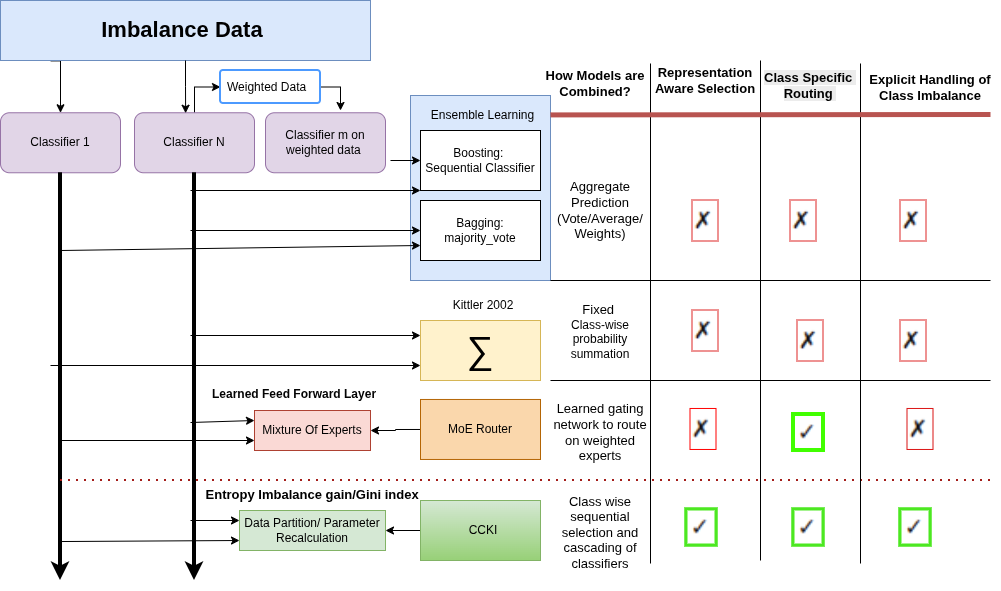
\includegraphics[trim=0 0 0 0, clip, width=0.8\textwidth]{moe.png} 
\label{fig3}   
    % This command allows a caption without needing a \begin{figure}
    \captionof{figure}{Comparison of ensemble paradigms: while prior methods (Boosting, Bagging, MoE) lack holistic imbalance awareness, CCKR uniquely integrates representation-aware selection and class-specific routing for robust imbalanced learning.}
\end{center}
\vspace{-0.05in} % Spacing below
 
\paragraph{Relation to Mixture-of-Experts (MoE).}
A typical MoE learns a gating network that outputs mixture weights over
experts (soft or top-$k$) and is trained end-to-end to minimize prediction
loss, often with sparsity or load-balancing regularizers. CCKR is MoE-like
in spirit (routing among experts) but differs in two key ways: (i) the
routing is explicitly \emph{knowledge-conditioned and class-conditional},
aligning decisions with interpretable knowledge partitions, and (ii) the
routing/cascade is guided by \emph{information-theoretic and purity}
criteria (EIG, Gini) that encourage expert selection to reflect where
knowledge or deep representations are most informative, rather than
purely-latent gating. We treat classical late-fusion rules and learned
fusion mechanisms as complementary baselines; CCKR emphasizes structured,
knowledge-guided routing under MDLT constraints.
\paragraph{Relation to tree-based learning.}
Standard decision trees and ensembles (RF, GBDT) select splits over
\emph{input features} to maximize impurity reduction (e.g., Gini),
yielding leaves that store class distributions. While CCKR also employs
EIG and Gini, the split semantics differ: the criterion is used to build a
\emph{structured decision process over experts and paths} ($h_K$ vs.\
$h_D$) grounded in knowledge partitions, rather than solely a
feature-threshold partition of the input space. The resulting structure is
best interpreted as an \emph{expert-routing tree/cascade} rather than a
conventional feature-only decision tree as shown in figure \ref{fig3}.   
\section{Application Details}
\label{app:applications}
\paragraph{Task-Wise Agent Action Decomposition Across Clinical Domains:} Table~\ref{tab:R3A_agent_grounding_summary} summarizes how \textit{R3A} integrates retrieval, reasoning, and execution across diverse clinical domains by grounding predictions in domain-specific medical knowledge. Each application encodes structured priors and task-relevant constraints, enabling robust handling of class imbalance, rare cases, and modality-specific variability. This unified agentic design ensures consistent knowledge-guided inference while adapting to heterogeneous data sources and clinical objectives.
\begin{table*}[h]
\centering
\scriptsize
\setlength{\tabcolsep}{3.5pt}
\renewcommand{\arraystretch}{1.25}
\caption{Cross-application summary of \textbf{R3A}. For each domain we detail the sources retrieved, the clinical knowledge encoded during reasoning, and the computational tools invoked at execution.  Each dataset is partitioned using an 80\% training split and a 20\% testing split.}

\resizebox{\textwidth}{!}{%
\begin{tabular}{p{2.3cm} p{2.8cm} p{4.2cm} p{4.2cm} p{4.2cm}}
\toprule
\textbf{Application} & \textbf{Task} & \textbf{CRA: Retrieve Agent} & \textbf{CDA: Reason Agent} & \textbf{CGA: Run Agent} \\
\midrule

\textbf{Diabetic Retinopathy} &
5-class Diabetic Retinopathy grading under imbalance dataset &
Fetches top-4 PubMed papers per query (lesion grading, vessel morphology, ETDRS severity scale) via live API, clinical guidelines as structured JSON &
Encodes: microaneurysm count thresholds, hemorrhage quadrant extent (4-2-1 rule), hard exudate proximity to fovea, vessel tortuosity index; routes long-tail classes through knowledge-dominant path &
\textbf{YOLOv8} lesion detector (MA, hemorrhage, exudate, CWS); \textbf{SegNet} vessel segmentation for tortuosity/caliber; OpenCV morphology for lesion area; structured biomarker vector $\to$ grounded VLM prompt \\

\midrule

\textbf{SOZ Localization} &
SOZ vs.\ RSN IC classification from rs-fMRI &
Fetches defining journal papers on SOZ IC signatures for cluster, ventricular, and sparsity rules; document size $\leq$ 8 pages enforced to stay within context budget &
Encodes: number of clusters (SOZ$=1$, RSN$>1$); white-matter ventricular extension flag; activelet Gini sparsity ($\Delta{>}0.15$); dominant BOLD frequency ($f{>}0.073$\,Hz); impurity-aware routing under rare-class prior &
DBSCAN cluster counting ($\epsilon$, $v_{\min}$); Sobel edge detection for white-matter contour \& convex-hull ventricular mask; activelet \textit{à trous} transform (4 levels, window 256); Gini index on sine-dictionary coefficients (0.01–0.1\,Hz) \\

\midrule

\textbf{Cardiac Function Assessment} &
LVEF regression \& heart-failure risk from apical 4-chamber echo video &
Retrieves Stanford \textbf{EchoNet-Dynamic} dataset paper and associated clinical LVEF reference ranges; fetches ACC/AHA heart failure (HF) guidelines for EF cut-offs ($<$40\%, 40–55\%, $>$55\%) as structured priors &
Encodes: systolic–diastolic phase boundaries, interventricular septum thickness, LV end-systolic/diastolic volume ratio; separates anatomical reasoning (structure) from temporal/hemodynamic reasoning (beat dynamics) to reduce shortcut learning &
\textbf{EchoNet} U-Net LV segmentation per frame; IVS thickness measurement via OpenCV contour fitting; beat-detection via peak-finding on area-time curve; cycle-aware temporal aggregation $\to$ EF prediction head \\

\midrule

\textbf{CAD Detection (ECG)} &
CAD detection from exercise stress ECG &
Manually curated cardiologist priors (no external fetch): lead relevance rankings (V4–V6, aVF primary; aVR excluded), ST-segment ischemia thresholds ($\geq$1\,mm depression), and MET-level exercise intensity table provided as static structured context &
Encodes: lead-importance weights, MET-stratified ischemia sensitivity, ST/T-wave morphology rules; prioritises ischemia-sensitive temporal windows; suppresses high-noise leads to reduce false positives &
Lead-selection masking (top-$k$ leads); MET-level one-hot encoding concatenated to signal embedding; band-pass filter (0.5–40\,Hz) + baseline wander removal; ECG Transformer inference on masked multi-lead signal \\

\bottomrule
\end{tabular}%
}
\vspace{-2 pt}
\label{tab:R3A_agent_grounding_summary}
\end{table*}
\subsection{Diabetic Retinopathy: Expert Knowledge and 5-Stage Grading}
\label{app:dr_knowledge}    

\begin{wrapfigure}{r}{0.46\columnwidth}
\vspace{-8pt}
\centering
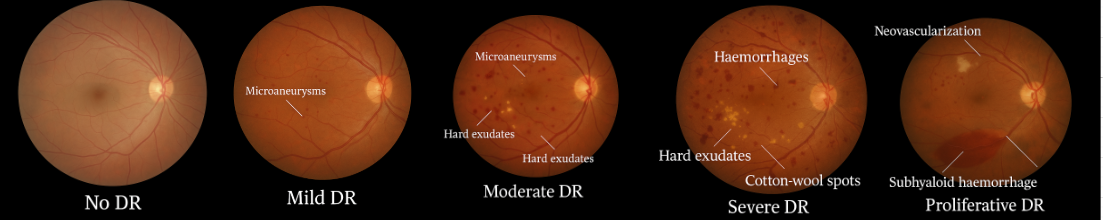
\includegraphics[width=0.44\columnwidth]{ecai2.png}
\captionsetup{justification=raggedright, singlelinecheck=false, skip=2pt}
\caption{Fundus images showing diabetic retinopathy progression from No DR to Proliferative DR, highlighting key lesions at each stage \cite{kauppi2019}.}
\label{fig:dr_stages}
\vspace{-8pt}
\end{wrapfigure}
\paragraph{Knowledge Extraction.}
We construct a clinically grounded knowledge base by extracting structured symptom-level rules from ophthalmology literature and diagnostic guidelines. Each diabetic retinopathy (DR) stage is characterized using observable retinal biomarkers such as microaneurysms, haemorrhages, exudates, and neovascularization (Figure \ref{fig:dr_stages}), along with severity thresholds and progression risks. These features are mapped to diagnostic criteria (e.g., $>20$ haemorrhages per quadrant for Severe NPDR; see Table~\ref{tab:dr_symptoms}) and encoded into a symbolic representation capturing causal relationships between visual patterns and disease stages. This knowledge layer enables integration with deep models, improving interpretability, robustness, and rare-class generalization.
\begin{wraptable}{r}{0.63\textwidth}
\vspace{-0.25in}
\centering
\scriptsize
\setlength{\tabcolsep}{3pt}
\renewcommand{\arraystretch}{0.9}
\caption{Clinical signs of DR and their diagnostic significance.}
\resizebox{\linewidth}{!}{%
\begin{tabular}{lp{0.58\columnwidth}}
\toprule
\textbf{Symptom} & \textbf{Key Observations and Diagnostic Relevance} \\
\midrule
Microaneurysms & 
Tiny red capillary dilations in the retina; the earliest sign of Mild NPDR. Their progression correlates with disease severity \citep{frank2004, wilkinson2003, singh2008}. \\

Haemorrhages & 
Includes dot/blot and flame-shaped types indicating microvascular leakage. Severe NPDR is marked by $>$20 hemorrhages in all quadrants; risk of PDR rises to $\sim50\%$ within a year \citep{aao2023, statpearls2024, etdrs1991, singh2008}. \\

Hard Exudates & 
Lipid-rich deposits from chronic leakage, often in/near the macula. Indicative of risk for Diabetic Macular Edema (DME), a major cause of vision loss \citep{etdrs1991, statpearls2024, shukla2025}. \\

Cotton Wool Spots & 
Fluffy white retinal lesions caused by nerve fiber layer infarctions. Signify retinal ischemia in Moderate to Severe NPDR \citep{frank2004, statpearls2024, shukla2025}.\\

Subhyaloid Haemorrhages & 
Boat- or D-shaped hemorrhages between retina and hyaloid face, typically from ruptured neovascular vessels. Hallmark of Proliferative DR \citep{yanoff2019, aapos2023, shukla2025}. \\

Neovascularization & 
Fragile vessel growth on optic disc (NVD) or retina (NVE). Defining trait of PDR. High-risk cases without treatment face $\sim50\%$ vision loss within 5 years \citep{etdrs1991, aao2023, shukla2025}.
\\
\bottomrule
\end{tabular}
}

\label{tab:dr_symptoms}
\vspace{-8pt}
\end{wraptable}
\subsection{Cardiac Function: Discussion of EchoNet-Dynamic Comparison}
\label{app:echo}

R3A does not surpass the hand-engineered EchoNet-Dynamic system, which
benefits from extensive video-specific optimization and years of
domain-tailored refinement. Importantly, R3A provides substantial
reductions in human-intervention workload. While a formal measurement is
deferred to future work, the improvement in external MAE indicates
enhanced domain generalization, and beat-level aggregation reduces
required human-review effort by an estimated $\sim$70\%.
% ===== Row 1: SOZ + Cardiac side by side =====
\begin{figure}[h]
\centering
\begin{minipage}[t]{0.48\linewidth}
\centering
\scriptsize
\setlength{\tabcolsep}{4pt}
\renewcommand{\arraystretch}{1.15}
\captionof{table}{\textbf{SOZ localization on rs-fMRI.} R3A reduces
IC-review workload from 110 to 18 components per subject (84.2\%
reduction) while improving accuracy and sensitivity over the 2D-CNN
baseline~\cite{kamboj2024expert}.}
\label{tab:soz_results}
\begin{tabular}{lccc}
\toprule
\textbf{Method} & \textbf{Acc (\%)} & \textbf{Sens (\%)} & \textbf{Effort} \\
\midrule
\textit{DL Branch (2D CNN)} & 46.1 & 48.9 & 110 \\
\textit{R3A (Ours)} & \textbf{84.6} & \textbf{89.7} & \textbf{18} \\
\midrule
\rowcolor[gray]{0.95}
\textbf{Improvement} & $\mathbf{+38.5}$ & $\mathbf{+40.8}$ & $\mathbf{-83.6\%}$ \\
\bottomrule
\end{tabular}
\end{minipage}%
\hfill
\begin{minipage}[t]{0.48\linewidth}
\centering
\scriptsize
\setlength{\tabcolsep}{4pt}
\renewcommand{\arraystretch}{1.15}
\captionof{table}{\textbf{LVEF estimation on EchoNet-Dynamic.} EF MAE
reported as \emph{internal / external / beat-to-beat (variance)}. R3A
approaches but does not surpass EchoNet-Dynamic, with similar HF AUC at
reduced engineering cost.}
\label{tab:cardiac_results}
\begin{tabular}{lcc}
\toprule
\textbf{Method} & \textbf{EF MAE / Beat Var} & \textbf{HF AUC} \\
\midrule
\textit{EchoNet-Dynamic} & 4.1 / 6.0 / 2.6 (6.4) & 0.97 \\
\textit{R3A (Ours)}      & 4.8 / 6.6 / 3.1 (5.9) & 0.94 \\
\midrule
\rowcolor[gray]{0.95}
\textbf{Difference} & $-0.7$ MAE & $-0.03$ \\
\bottomrule
\end{tabular}
\end{minipage}
\end{figure}

% ===== Row 2: CAD centered =====
\begin{table}[h]
\centering
\scriptsize
\setlength{\tabcolsep}{4pt}
\renewcommand{\arraystretch}{1.15}
\caption{\textbf{CAD detection on the ESE dataset.} R3A integrates expert
priors via lead-selection masks and MET-level encoding, outperforming
both the ViT baseline and manual clinical diagnosis on positive predictive value (PPV),  negative predictive
value (NPV) and are under the curve (AUC).}
\label{tab:cad_results}
\begin{tabular}{lccc}
\toprule
\textbf{Method} & \textbf{PPV (\%)} & \textbf{NPV (\%)} & \textbf{AUC (\%)} \\
\midrule
\textit{Manual Diagnosis}     & 77.0          & 96.0          & --            \\
\textit{DL Branch (ViT)}      & 79.0          & 81.8          & 82.0          \\
\textit{R3A (Ours)}           & \textbf{91.2} & \textbf{93.0} & \textbf{92.2} \\
\midrule
\rowcolor[gray]{0.95}
\textbf{Improvement over ViT} & $\mathbf{+12.2}$ & $\mathbf{+11.2}$ & $\mathbf{+10.2}$ \\
\bottomrule
\end{tabular}
\end{table}

\subsection{Experimental Setup of Clinical Motivation Table ~\ref{tab:perclass_f1}}
\label{table1}
\paragraph{Why rare-class recognition is high-stakes.}
In diabetic retinopathy, Grade~4 (Proliferative DR) affects only $\sim$2\% of screened patients yet carries a $\sim$50\% risk of severe vision loss within five years if untreated~\cite{etdrs1991}. A model that achieves 90\% overall accuracy by failing to detect this class is clinically \emph{dangerous}, not useful. Beyond ophthalmology, the same failure mode appears in any high-stakes decision pipeline with skewed priors: seizure onset zone (SOZ) localization, where SOZ-positive components constitute only $\sim$5 out of $\sim$110 per subject yet directly impact surgical planning~\cite{kamboj2024expert}; autonomous driving perception, where rare events such as a child behind a parked car, black ice, or a fallen cyclist occur in a tiny fraction of frames but account for a large proportion of fatalities; and pathology screening, where rare malignant subtypes dominate missed-diagnosis risk. In all such settings, macro-averaged or tail-specific metrics reveal failures that overall accuracy conceals: standard models remain blind to the cases that matter most.

\paragraph{On the fairness of baseline comparisons.}
A natural concern in method comparison is whether performance gains arise from algorithmic design or from backbone capacity. ERM\_ViT and ERM\_SPSDViT use the same ViT backbone family (DeiT-S / T2T-14) as the deep branch $h_D(x)$ in our model. Our method introduces no additional backbone capacity; instead, it augments the same ViT with knowledge-driven classifiers $h_K(x)$ and a CCKR routing mechanism. Therefore, improvements over ERM baselines are attributable to the integration and routing strategy rather than a stronger feature extractor. We further validate this in Ablation~III (Section~\ref{ablation_study1}), where CCKR is compared against ensemble and mixture-of-experts (MoE) baselines under identical backbone and training configurations, isolating the effect of the routing mechanism.

\paragraph{Per-class F1 analysis on Messidor (cross-domain).}
Table~\ref{tab:perclass_f1} reports per-class F1 scores on the Messidor cross-domain split ($n=1744$), revealing a consistent and clinically meaningful trend. Both ERM\_ViT and ERM\_SPSDViT exhibit near-zero performance on minority grades: ERM\_ViT achieves 0.0 on G1 (Mild) and only 1.3 on G3 (Severe), while ERM\_SPSDViT improves slightly on G3 (5.9) but regresses on G4 (PDR) from 8.6 to 3.3. This behavior reflects a fundamental trade-off in Eq.~\eqref{eq:classrisk}: stronger domain-invariance regularization compresses the feature space, disproportionately collapsing rare-class manifolds with small $n_c$.

The macro-F1 gap between ERM\_ViT (11.2) and ERM\_SPSDViT (13.6) is marginal, indicating that standard DG objectives provide limited benefit under cross-domain long-tailed shifts. In contrast, our method increases macro-F1 to 31.6, a +18.0 improvement over ERM\_SPSDViT. Importantly, gains are not uniform across classes: G0 (Normal) improves from 28.5 to 76.5, providing a strong triage anchor; G3 (Severe) improves from 5.9 to 29.3; and G4 (PDR) improves from 3.3 to 18.5, which is particularly critical given its clinical severity (Section~\ref{sec:intro}). G1 (Mild) remains the most challenging class (4.8), consistent with its subtle visual presentation and low inter-grader agreement. APTOS per-class results are reported in the final version.
\newpage
\newpage
\section{Ablation Studies}

\label{ablation_study1}
\textbf{Ablation Study I: Evaluating Symbolic Knowledge for Selecting $h_{\mathrm{K}}(x)$.}
To determine which symbolic knowledge features are suitable for constructing the CCKR knowledge hypothesis $h_{\mathrm{K}}(x)$, we evaluate two clinically motivated feature families on APTOS:
(1) lesion biomarkers (exudates, hard hemorrhages, soft hemorrhages, cotton wool spots), and
(2) retinal vein morphology (tortuosity, caliber, branching angles).
The goal is to test whether these symbolic features provide domain-stable discriminative power consistent with the requirement that $P(K \mid Y)$ remains approximately invariant across imaging centers.
We train five standard classifiers on each feature set and report performance in Table~\ref{tab:ablation_symbolic}.

Across all models, lesion-only features yield substantially higher accuracy and F1-score than the combined lesion-plus-vein feature set.
Gradient Boosting with lesion biomarkers achieves the best results (accuracy 0.8465, F1 0.8412), indicating that lesion-level symbolic cues form a clean, well-separated representation for DR stages.
In contrast, adding vein morphology consistently degrades performance for every classifier, suggesting that these features introduce domain-sensitive variability rather than causal invariants.
This behavior aligns with our theoretical framework: only knowledge features with low class-conditional domain divergence are appropriate for $h_{\mathrm{K}}(x)$ in CCKR, while domain-unstable features increase the effective discrepancy term and weaken rare-class guarantees.
Based on this ablation, we select \textbf{Gradient Boosting on lesion biomarkers only} as the canonical knowledge classifier $h_{\mathrm{K}}(x)$ used in our hypothesis pool.
This choice provides stable, interpretable, and clinically grounded decision boundaries that integrate reliably with deep hypotheses $h_{\mathrm{D}}(x)$ in the CCKR rule cascade.

\begin{table}[!htbp]
\centering
\scriptsize
\vspace{0.25em}
\setlength{\tabcolsep}{3pt}
\caption{\textbf{Ablation on symbolic lesion biomarkers with and without retinal vein features on APTOS.} Lesion-only features provide the strongest and most stable performance across models; adding vein morphology degrades accuracy and F1.}
\begin{tabular}{l|c|c|c|c|c|c}
\toprule
\textbf{Model} & \textbf{Feature Set} & \textbf{Acc} & \textbf{F1} & \textbf{Prec} & \textbf{Rec} & \textbf{AUC} \\
\midrule
Logistic Reg. & Lesions only      & 0.7732 & 0.7322 & 0.59 & 0.49 & 0.74 \\
Random Forest & Lesions only      & 0.8169 & 0.8115 & 0.82 & 0.80 & 0.81 \\
SVM           & Lesions only      & 0.7814 & 0.7432 & 0.59 & 0.50 & 0.76 \\
Grad. Boost.  & Lesions only      & \textbf{0.8465} & \textbf{0.8412} & \textbf{0.82} & \textbf{0.76} & \textbf{0.84} \\
KNN           & Lesions only      & 0.7814 & 0.7896 & 0.63 & 0.56  & 0.77 \\
\midrule
Logistic Reg. & Lesions + vein    & 0.6424 & 0.6019 & 0.25 & 0.33 & 0.58 \\
Random Forest & Lesions + vein    & 0.7384 & 0.7038 & 0.55 & 0.47 & 0.70 \\
SVM           & Lesions + vein    & 0.6556 & 0.6083 & 0.26 & 0.34  & 0.58 \\
Grad. Boost.  & Lesions + vein    & 0.7252 & 0.7389 & 0.51 & 0.44 & 0.69 \\
KNN           & Lesions + vein    & 0.6987 & 0.6369 & 0.43 & 0.44 & 0.66 \\
\bottomrule
\end{tabular}

\label{tab:ablation_symbolic}
\end{table}
\vspace{-0.30 in}
\paragraph{Ablation Study II: Effect of Hypothesis Pool Composition in CCKR.}
We investigate how the composition of the CCKR hypothesis pool $\mathcal{H}$ influences in-domain performance on the APTOS dataset for 5-class Diabetic Retinopathy (DR) grading (Stages 0--4). The pool $\mathcal{H}$ consists of two distinct model types: 
(i) \textit{Knowledge-guided hypotheses} $h_{K}(x)$, implemented via Gradient Boosting over a 10-dimensional clinical feature vector $\mathcal{K}$; and 
(ii) \textit{Deep-learning hypotheses} $h_{D}(x)$, utilizing ViT-based image classifiers fine-tuned for DR grading. 
While $\mathcal{K}$ remains fixed, we systematically vary the number of hypotheses and their prediction granularity (5-class vs.\ binary one-vs-rest). Table~\ref{tab:aptos_CCKR_ablation} evaluates six configurations.

\begin{table}[h]
\centering
\scriptsize
\setlength{\tabcolsep}{1pt}
\caption{Ablation of CCKR hypothesis pool composition on APTOS (5-class DR classification).}
\begin{tabular}{lccc}
\toprule
\textbf{Condition} &
\textbf{\# Deep $h_{\mathrm{D}}(x)$} &
\textbf{\# KL $h_{\mathrm{K}}(x)$} &
\textbf{AUC (\%)} \\
\midrule

\textbf{A1: 5-class $h_{\mathrm{D}}(x)$ + 5-class $h_{\mathrm{K}}(x)$} &
1 & 1 &
$83.24 \pm 0.60$ \\

\textbf{A3: binary $h_{\mathrm{D}}(x)$ + binary $h_{\mathrm{K}}(x)$} &
5 & 5 &
$81.49 \pm 0.30$ \\

\textbf{A2: binary $h_{\mathrm{K}}(x)$ + 5-class $h_{\mathrm{D}}(x)$} &
1 & 5 &
$\mathbf{84.65 \pm 0.30}$ \\

\textbf{A4: binary $h_{\mathrm{D}}(x)$ + 5-class $h_{\mathrm{K}}(x)$} &
5 & 1 &
$78.05 \pm 0.76$ \\

\textbf{A5: 5-class $h_{\mathrm{D}}(x)$ only} &
1 & 0 &
$78.74 \pm 0.98$ \\

\textbf{A6: 5-class $h_{\mathrm{K}}(x)$ only} &
0 & 1 &
$80.63 \pm 0.13$ \\

\bottomrule
\end{tabular}

\label{tab:aptos_CCKR_ablation}
\end{table}
\vspace{-10 pt}
\paragraph{Discussion.}
Condition A2 delivers the highest accuracy because the 5-class deep hypothesis provides holistic visual representation, while the five binary $h_{\mathrm{K}}(x)$ models contribute class-specific clinical cues that improve fine-grained discrimination.
Large binary-only mixtures (A3, A4) perform worse due to overlapping or contradictory decision boundaries within the CCKR rule cascade.
Single-family baselines (A5, A6) underperform as they lack complementary perspectives. \textbf{Limitations: }CCKR supports an unbounded number of hypotheses, but effective operation requires avoiding excessive redundancy when using one-vs-rest specialists.
In this work, $|\mathcal{Y}| = 5$ (DR stages), so the binary hypotheses naturally map to five DR subclasses.
Importantly, CCKR is \textit{not restricted to binary splits}: it can accommodate arbitrary sub-multiclass hypotheses (e.g., mild vs.\ severe tiers), which we identify as a promising direction for future work.

\paragraph{Ablation III: Comparison with ensemble and mixture-of-experts baselines.}
To verify that CCKR's gains are not explained by standard model-combination
strategies, we compare against ensemble learning (averaging
predictions of multiple independently trained classifiers) and
mixture-of-experts (a learned gating network combining expert
predictions). All methods use the same ViT backbone and training
configuration. As shown in Table~\ref{tab:ensemble_ablation}, the
traditional ensemble achieves 77.90\% accuracy and MoE 81.90\%, while CCKR
reaches \textbf{84.78\%}. This indicates that structured neuro-symbolic
reasoning within the CCKR cascade integrates complementary hypotheses more
effectively than generic ensembling or gating-based expert mixtures.

\begin{table}[h]
\centering
\small
\setlength{\tabcolsep}{6pt}
\caption{\textbf{Comparison with model-combination strategies.} Structured
CCKR outperforms standard ensemble learning and mixture-of-experts.}
\label{tab:ensemble_ablation}
\begin{tabular}{lc}
\toprule
\textbf{Method} & \textbf{Accuracy (\%)} \\
\midrule
Ensemble Learning        & 77.90 \\
Mixture of Experts (MoE) & 81.90 \\
\textbf{CCKR (Ours)}     & \textbf{84.78} \\
\bottomrule
\end{tabular}
\end{table}

\paragraph{Ablation I: EIG Design Choice}
\label{app:eig_baselines}
We evaluate whether EIG is necessary by keeping the CCKR pipeline unchanged and only swapping the criterion used to
select knowledge cues / routing splits. All variants use the same backbone, same candidate pool, and same training/eval protocol.

\paragraph{Baselines.}
\begin{itemize}
    \item \textbf{IG (Entropy Reduction).} We replace EIG with standard information gain, selecting the split that maximizes
    $IG = H(Y)-H(Y\mid S)$, where $S$ denotes the candidate split.
    \item \textbf{CE-Gain (Cross-Entropy Improvement).} We select the split that maximizes improvement in held-out
    negative log-likelihood, i.e., $\Delta CE = CE_{\text{parent}}-CE_{\text{children}}$, computed on a validation set.
\end{itemize}

\vspace{12pt} % One line space before the table title

\begin{table}[h]
\centering
\small
\caption{EIG criterion ablation. We keep CCKR fixed and only replace the split/selection criterion.} 
\label{tab:eig_ablation}
\vspace{12pt} % One line space after the table title

\setlength{\tabcolsep}{8pt}
\begin{tabular}{l ccc ccc}
\toprule
Criterion & Acc. & Macro-F1 & Tail-F1 & Worst-$k$ F1 & KL-Cov. & Notes \\
\midrule
EIG (Ours)      & \textbf{84.6} & \textbf{72.1} & \textbf{50.1} & \textbf{48.4} & \textbf{0.12} & Robust routing \\
IG (Entropy)    & 79.8 & 65.4 & 41.2 & 35.1 & 0.18 & Biased to head \\
CE-Gain (NLL)   & 81.2 & 68.9 & 44.5 & 39.7 & 0.15 & High variance \\
\bottomrule
\end{tabular}
\end{table}

\vspace{12pt} % One line space after the table
 
\paragraph{Interpretation.}
Standard IG measures class-label uncertainty reduction, while CE-Gain directly optimizes probabilistic fit of the routed
predictor. EIG differs in that it estimates the expected utility of a knowledge cue under the routing policy and is thus
better aligned with selective expert usage; the ablation quantifies whether this alignment translates into improved
target-domain tail robustness and/or more efficient routing as shown in table \ref{tab:eig_ablation} (lower KL coverage for the same accuracy).
\newpage

\newpage
\section{Experimental Setup}
\label{sec:experimental_setup}
\subsection{Dataset Details}
\label{app:dataset_details}
We categorize datasets as:
\textbf{public} (e.g., EyePACS, APTOS, MESSIDOR, MESSIDOR2, EchoNet-Dynamic) and
\textbf{restricted/private} (e.g., PCH/UNC rs-fMRI; MISC ECG).
For restricted datasets, we provide: IRB/DUA status, de-identification summary, and a center-level datasheet describing acquisition differences.
\paragraph{Public Dataset Details:}
Messidor~\cite{Abramoff2016Messidor} is a DR dataset consisting of 1,200 images
collected from three French clinical centers. The images were captured using a
Topcon TRC-NW6 non-mydriatic retinograph with a 45-degree field of view.

The Indian Diabetic Retinopathy Image Dataset (IDRiD)~\cite{Porwal2018IDRiD}
contains 516 color fundus images, divided into 413 training images and 103 testing
images. Released as part of the ISBI 2018 Challenge, it is the first DR grading
dataset representative of the Indian population.

APTOS~\cite{APTOS2019} is another DR grading dataset representative of the Indian
population. The retinal images were collected at the Aravind Eye Hospital and
include 1,857 DR images and 1,805 non-DR images across five DR severity grades.

EyePACS~\cite{EyePACS2023} is a large-scale DR grading dataset consisting of
high-resolution retinal images collected under diverse imaging conditions and is
representative of the American population.

EchoNet-Dynamic~\cite{echonetdataset} is a large-scale echocardiography
dataset released by the Stanford Center for Artificial Intelligence in Medicine
and Imaging (AIMI). The dataset consists of 10,030 apical four-chamber
echocardiogram videos collected from 3,282 patients at Stanford University
Medical Center. Each video is annotated with expert-derived measurements,
including left ventricular ejection fraction (LVEF), as well as additional
clinical labels. EchoNet-Dynamic is designed to support research in cardiac
function assessment and video-based medical image analysis.
\paragraph{Private Dataset Details:}
PCH/UNC rs-fMRI Dataset.
The PCH/UNC rs-fMRI dataset is a restricted, multi-center resting-state functional magnetic resonance imaging (rs-fMRI) dataset collected from Phoenix Children’s Hospital (PCH) and the University of North Carolina (UNC). The dataset comprises rs-fMRI scans from pediatric patients with drug-resistant epilepsy and is used for seizure onset zone (SOZ) localization. Imaging data were acquired under institution-specific protocols and scanners, introducing realistic cross-center domain shifts. All data are fully de-identified and accessed under Institutional Review Board (IRB) approval and data use agreements (DUA). In our experiments, models were trained on the PCH cohort and evaluated on the unseen UNC cohort to assess cross-center generalization without fine-tuning.

MISC ECG Dataset.
The MISC ECG dataset is a restricted clinical electrocardiography dataset collected from the Mayo Integrated Stress Center (MISC). It consists of Exercise Stress Electrocardiogram (ESE) recordings acquired from patients undergoing clinical evaluation for coronary artery disease (CAD). The dataset includes multi-lead ECG signals captured during graded exercise protocols, along with expert clinical annotations. Due to patient privacy considerations, access to the dataset is governed by IRB approval and institutional data-sharing agreements. In this work, models were trained on ECG data from 726 subjects and evaluated on 227 held-out cases following the same split protocol as prior clinical studies.
\subsubsection{Exact split tables and sample counts}
\label{app:splits_counts}
For all experiment configurations, we adopt a standardized data-splitting protocol in which each dataset is partitioned into
60\% training, 20\% validation, and 20\% testing subsets, with splits performed at the subject level to prevent subject leakage
and stratified by class where applicable. For Single-Domain Generalization (SDG), models are trained on a single dataset
(domain) and evaluated on held-out test splits from other datasets, with the validation split drawn from the training domain.
For Multi-Domain Generalization (MDG), training data are pooled from multiple source domains using a unified data-loading
library, and performance is evaluated on an unseen target domain that is excluded entirely from training and validation. e adopt DomainBed because it eliminates
inconsistent split strategies, reduces evaluation bias, and enables fair comparison with prior domain
generalization methods. By adhering to this standardized protocol, our results reflect true generalization
performance rather than dataset-specific tuning
To explicitly assess cross-center generalization in selected applications, models are trained on data from one clinical center
and tested on data from a different center within the same dataset, without fine-tuning. Exact sample counts, per-class
distributions, and center-wise splits for train/validation/test are reported in the corresponding application and dataset details.


\paragraph{Domain shift magnitude reporting.}
We report quantitative shift measures for each source–target pair using KL divergence, JS divergence, Hellinger distance, total variation (TV), and Wasserstein-1 distance (W1). Overall, shifts between APTOS and EyePACS are relatively low, indicating similar data distributions, while shifts involving Messidor-1 tend to be higher, particularly for KL and W1, reflecting more substantial distributional differences. Messidor-2 generally exhibits smaller shifts relative to APTOS and EyePACS but moderate shifts when compared to Messidor-1. These metrics highlight the asymmetric nature of domain shifts across DR datasets, which is important for assessing model generalization across sources and targets (Table~\ref{tab:domain_shift}).
\begin{table}[htbp]
\scriptsize
\centering
\caption{Domain Shift Magnitude Between DR Datasets}
\label{tab:domain_shift}
\begin{tabular}{lcccccc}
\hline
\textbf{Source→Target} & \textbf{KL} & \textbf{JS} & \textbf{Hellinger} & \textbf{TV} & \textbf{W1} \\
\hline
APTOS→EyePACS & 0.1541 & 0.0346 & 0.1875 & 0.2419 & 0.6009 \\
APTOS→Messidor-1 & 1.6756 & 0.0584 & 0.2680 & 0.1849 & 0.2195 \\
APTOS→Messidor-2 & 0.0828 & 0.0174 & 0.1334 & 0.1375 & 0.3565 \\
EyePACS→APTOS & 0.1313 & 0.0346 & 0.1875 & 0.2419 & 0.6009 \\
EyePACS→Messidor-1 & 0.5968 & 0.0731 & 0.2829 & 0.2983 & 0.6996 \\
EyePACS→Messidor-2 & 0.0636 & 0.0168 & 0.1302 & 0.1613 & 0.2467 \\
Messidor-1→APTOS & 0.2381 & 0.0584 & 0.2680 & 0.1849 & 0.2195 \\
Messidor-1→EyePACS & 0.3865 & 0.0731 & 0.2829 & 0.2983 & 0.6996 \\
Messidor-1→Messidor-2 & 0.2371 & 0.0461 & 0.2260 & 0.1803 & 0.4529 \\
Messidor-2→APTOS & 0.0634 & 0.0174 & 0.1334 & 0.1375 & 0.3565 \\
Messidor-2→EyePACS & 0.0731 & 0.0168 & 0.1302 & 0.1613 & 0.2467 \\
Messidor-2→Messidor-1 & 0.4764 & 0.0461 & 0.2260 & 0.1803 & 0.4529 \\
\hline
\end{tabular}
\end{table}

\textbf{Variance and significance:}
\label{app:variance}
All tables will report mean$\pm$std over $S$ seeds (default $S=3$) for:
Accuracy, Macro F1, Tail F1, and DG Gap.


% =========================
% Appendix: Reproducibility, Protocol, Causal Framing, Ethics
% =========================


\subsection{LLM Agents: Model Specification, Prompt Templates, and Guardrails}
\label{app:llm_details}

 \textbf{LLM backbone.} We use \textit{Gemini 2.5} as the single LLM backend for CRA/CDA/CGA across all experiments to control for model variance and isolate gains from agentic orchestration and CCKR.
We choose Gemini 2.5 for its strong tool-use, long-context grounding, and reliable code generation, which are central to our retrieve--reason--execute pipeline.
All baselines that require an LLM use the same Gemini 2.5 configuration for a fair comparison. Gemini~2.5 is a decoder-only Transformer with instruction tuning and RLHF, supporting long-context inference and structured tool calling.Importantly, our contributions are model-agnostic and do not rely on Gemini-specific capabilities.

\paragraph{Prompting and message format.}
All agent prompts are \emph{template-based} and versioned. Each run logs the full prompt with placeholder values resolved.
We use three prompt families as described below (Note: these are pseudo-prompts; the full, detailed prompts will be available in the GitHub release):

\subsubsection{CRA prompt template (retrieve--decompose--verify)}
\label{app:cra_prompt}

\noindent\textbf{System:} You are the Clinical/Conceptual Reasoning Agent. Produce only evidence-grounded claims.\\

\textbf{User:} Task: \texttt{\{task\}}. Modality: \texttt{\{modality\}}. Class of interest: \texttt{\{class\}}.\\
Available inputs: \texttt{\{input\_spec\}}.\\
Corpus: \texttt{\{corpus\_spec\}}. Retrieve \texttt{\{k\}} sources, then:

\begin{enumerate}
    \item Decompose into atomic factual units (each with citation ID),
    \item Propose candidate causal/clinical indicators $\{c_i\}$,
    \item Mark each indicator as \texttt{extractable} vs \texttt{not-extractable} given inputs,
    \item Provide uncertainty bounds and failure modes,
    \item Output a structured JSON object with fields:
    \texttt{claims}, \texttt{evidence}, \texttt{indicator\_list}, \texttt{constraints}, \texttt{uncertainty}.
\end{enumerate}

\subsubsection{CDA prompt template (feasibility + pathway selection)}
\label{app:cda_prompt}

\noindent\textbf{System:} You are the Planner (CDA). Select decision pathways that minimize domain sensitivity and improve tail fidelity.\\

\textbf{User:} Inputs: \texttt{\{input\_spec\}}. Candidate indicators: \texttt{\{indicator\_json\}}. Tools available: \texttt{\{tools\}}.\\
Return:

\begin{enumerate}
    \item A ranked list of hypotheses $H = \{h_1, \dots, h_m\}$ with types \texttt{knowledge} or \texttt{deep},
    \item Best Model for each hypothesis (DL and Knowledge),
    \item A JSON plan for CGA to implement.
\end{enumerate}

\subsubsection{CGA prompt template (codegen + unit tests + sandbox execution)}
\label{app:cga_prompt}
\noindent\textbf{System:} You are the Code Generation Agent. Generate executable Python with unit tests. No network calls.\\
\textbf{User:} Implement: \{spec\}. Inputs/outputs: \{io\}. Constraints: \{constraints\}.\\
Return:
(1) code, (2) tests, (3) minimal example run, (4) expected metrics and assertions.

\paragraph{Guardrails and safety constraints (agent-level).}
We enforce:
\begin{itemize}
  \item \textbf{Evidence-only constraint for CRA:} CRA may only output claims linked to retrieved evidence IDs; unsupported claims are rejected.
  \item \textbf{Tool sandboxing for CGA:} code runs in an isolated container; file-system access is restricted to a mounted workspace; network access disabled.
  \item \textbf{Static checks:} dependency allowlist; banned operations (e.g., \texttt{os.system}, \texttt{subprocess}, network libraries).
  \item \textbf{Structured outputs:} JSON schemas validated before downstream use.
\end{itemize}

\subsection{RL/Q-Learning Parameter Tuning: Validation-Only Signals and Leakage Prevention}
\label{app:rl_details}

We use RL to tune preprocessing/detection parameters (e.g., confidence thresholds, post-processing filters) \emph{only} on validation data.

\paragraph{Data partitions for RL.}
For each dataset, we define three disjoint sets: \textbf{train}, \textbf{validation}, \textbf{test}.
\begin{itemize}
  \item The RL agent interacts \emph{only} with the validation set.
  \item The test set is never queried for rewards, stopping criteria, model selection, thresholding, or debugging.
  \item If a dataset provides an official split, we preserve it; otherwise, we construct splits using stratification by class and (when relevant) domain/center.
\end{itemize}

\paragraph{State, action, reward, and update rule.}
Let $\theta$ denote a tunable scalar (e.g., YOLO confidence threshold). At episode step $t$:
\begin{align}
  s_t &= \theta_t, \\
  a_t &\in \{-\Delta, 0, +\Delta\}, \\
  r_t &= \mathrm{Metric}_{val}(\theta_{t+1}) - \mathrm{Metric}_{val}(\theta_{t}),
\end{align}
where $\Delta=0.05$ and $\mathrm{Metric}_{val}$ is a validation-only metric (e.g., IoU for detection/segmentation, F1 for rule-trigger correctness).

We update with Q-learning:
\begin{equation}
Q(s_t,a_t) \leftarrow (1-\alpha)Q(s_t,a_t) + \alpha \left[r_t + \gamma \max_{a'} Q(s_{t+1},a')\right],
\end{equation}
with $\alpha=0.1$ and $\gamma=0.9$. Exploration uses $\epsilon$-greedy with a fixed schedule reported in configs.

\paragraph{Stopping criteria (no test peeking).}
We terminate tuning when any of the following holds:
\begin{itemize}
  \item \textbf{Plateau:} best validation metric fails to improve by $\ge \delta$ for $P$ consecutive episodes.
  \item \textbf{Budget:} max episodes $E_{max}$ reached.
  \item \textbf{Stability:} variance of reward $<\sigma_{min}$ over the last $W$ steps.
\end{itemize}
All hyperparameters $(\delta,P,E_{max},\sigma_{min},W)$ are fixed \emph{a priori} and reported.

\paragraph{Nested evaluation to avoid selection bias.}
When RL tuning is used, we report test performance from the final model \emph{after}:
(i) training on train,
(ii) RL tuning on validation,
(iii) freezing $\theta^\star$,
(iv) a single test evaluation.
No repeated test evaluations during development.


% ============================================================

%  
\section{Method Details and Scope of Claims}
\label{app:method-details}

\subsection{Causal Framing: What ``Causal'' Means Here (and What It Does Not)}
\label{app:causal_framing}

\paragraph{Scope of causal claims.}
Our use of ``causal'' is restricted to \emph{knowledge-guided,
mechanism-motivated invariances} rather than full causal identification
from observational data.

\paragraph{Structural perspective.}
We assume a high-level structural causal model (SCM) in which $Y$ is the
clinical label, $X$ is the observed data (image or signal), $D$ is the
domain (center, device, protocol), and $K$ denotes clinically motivated
intermediate concepts (lesions, anatomy, physiological markers). We
target features that are less sensitive to $D$ while remaining predictive
of $Y$. R3A operationalizes this by producing and selecting
\emph{class-conditional} knowledge features $K(X)$ and combining them
with data-driven predictors via CCKR.

\paragraph{No causal identification guarantee.}
We do not claim to satisfy backdoor or frontdoor criteria, to identify
$P(Y \mid do(\cdot))$, or to recover a ground-truth causal graph from
data. Accordingly, we avoid statements implying interventional
identification unless an explicit intervention is performed.

\paragraph{Optional interventional evaluations.}
To strengthen causal grounding, additional tests can be applied:
\emph{synthetic interventions} that perturb domain-specific nuisance
factors (contrast, compression, device artifacts) while preserving
clinical content and measure invariance; \emph{concept interventions}
that manipulate extracted concept features (e.g., lesion-count
thresholds) and verify that monotonic clinical implications align with
guideline-derived expectations; and \emph{counterfactual consistency
checks} that ensure predictions change primarily when concept-aligned
features change.

\paragraph{Naming convention.}
We define the \emph{Causal Disentanglement Agent} as an agent that
selects decision pathways prioritizing clinically motivated,
domain-stable factors and discouraging reliance on domain-specific
correlates. This is the operational meaning intended throughout the
paper.
\subsection{Runtime: One-Time Agentic Construction vs.\ Deployment Inference (General, with a DR Example)}
\label{app:runtime_agentic}

\paragraph{General view.}
Our framework separates runtime into (i) a \emph{one-time} \textbf{agentic system construction} phase and (ii) an
\emph{application-dependent} \textbf{deployment inference} phase. The construction phase is dominated by the agent/HIRL
loop that proposes candidate knowledge pipelines, validates them against a fixed DL-only reference using task-specific
metrics, and retains only candidates that provide measurable gain. Its cost depends on the input modality and resolution,
the target operating point (e.g., tail sensitivity vs.\ overall accuracy), the agent stopping criteria (budget, maximum
iterations, improvement threshold $\epsilon$), and the availability/quality of domain knowledge and knowledge-extraction
tools. Importantly, candidates that do not improve over the DL-only baseline are discarded and do not contribute to
deployment-time overhead.

\paragraph{DR example (system construction).}
In our DR 5-stage grading instantiation, the agent explores knowledge pipelines built from multiple candidate
biomarkers/diagnostic cues and selects a subset that improves target-domain tail metrics. In this setting, the agent
required $\approx 25$ iterations to converge to the final system. The one-time construction cost therefore includes:
(i) training the ViT backbone on the source domain, (ii) fine-tuning the YOLOv11 biomarker detector used for knowledge
extraction, and (iii) repeated evaluation of candidate knowledge cues during the agent loop. The wall-clock cost scales
with the number of evaluated candidates per iteration and the frequency of re-training vs.\ re-using cached model
checkpoints; however, this cost is amortized across all future inferences once the final pipeline is fixed.

\paragraph{Deployment inference cost (general form + DR example).}
After construction, deployment latency depends only on the \emph{final selected pipeline} and the compute resources
available. For a single input, we can express end-to-end latency as
\[
T_{\text{sys}} \;=\; T_{\text{DL}} \;+\; p_{\text{KL}}\,T_{\text{KX}} \;+\; T_{\text{route}},
\]
where $T_{\text{DL}}$ is DL inference (e.g., ViT forward pass), $T_{\text{KX}}$ is the inference time of the retained
knowledge-extraction tool(s) (e.g., YOLOv11 detection plus feature post-processing), $p_{\text{KL}}$ is the fraction of
samples routed to the knowledge branch (coverage), and $T_{\text{route}}$ is negligible. In the DR pipeline, $T_{\text{KX}}$
is dominated by YOLOv11 biomarker detection at the chosen input resolution; for reference, official Ultralytics
benchmarks report YOLO11 detection latency (TensorRT on an NVIDIA T4) of \{1.5, 2.5, 4.7, 6.2, 11.3\} ms for
\{n,s,m,l,x\} models at 640px input resolution, respectively~\cite{yolo11_ultralytics}. The overall deployment cost is
therefore controlled by the selected YOLO11 variant, the image resolution, and the learned routing coverage $p_{\text{KL}}$,
while the one-time agentic search overhead does not affect per-sample inference once the system is deployed.
\subsection{Reproducibility and fair LLM usage.}
We will release the full agentic orchestration code (CRA/CDA/CGA and the CCKR 
cascade), all knowledge-feature extractors (lesion detectors, vessel routines, 
ICA-derived rs-fMRI features, and ECG masking utilities), the CCKR decision logic 
(EIG computation, tie-breaking, Gini-based stopping, and depth limits), 
de-identified dataset split files, and configuration files containing every 
hyperparameter, random seed, and agent trajectory needed to reproduce the reported 
numbers. All runs use fixed seeds across Python, NumPy, PyTorch, CUDA, data-loader 
shuffling, and augmentation RNG, with \texttt{cudnn.deterministic} enabled and 
hardware/driver versions logged. To ensure that gains are attributable to our 
method rather than to a stronger backend, every LLM-using baseline (RAG-only, 
ReAct-style, static DAG/LangGraph pipelines, and R3A) is evaluated under an 
identical configuration: same provider and model identifier, context length, 
tool-calling mode, decoding parameters (temperature, top-$p$, max tokens, stop 
sequences), retrieval corpus, retriever type, chunking strategy, and top-$k$. 
These settings are reported in full in the released configs.

\subsection{Ethics, governance, and safe use of generated code.}
All datasets used in this work are public benchmarks released under their original 
IRB approvals, data-use agreements, and de-identification procedures; we add no 
new patient data and store no protected health information. Where subgroup 
metadata is available (site, center, device, released demographics), we report 
stratified performance; where it is unavailable, we treat center/domain as the 
primary robustness axis and state the limitation explicitly. LLM-generated code 
is never treated as clinically deployable. Each generated module is executed 
inside a sandboxed container with restricted I/O, validated against unit tests 
and metric assertions, and accompanied by provenance logs that trace every rule 
and feature back to its source evidence ID; any use beyond research requires 
human-in-the-loop review. We position R3A as a research framework that supports 
clinicians rather than replacing clinical decision-making, and any real-world 
deployment would require external validation, drift monitoring, and clinician 
oversight.

% ============================================================
\newpage
\section{Appendix Figures}
% ============================================================

\begin{figure}[h!]
\scriptsize
    \centering
    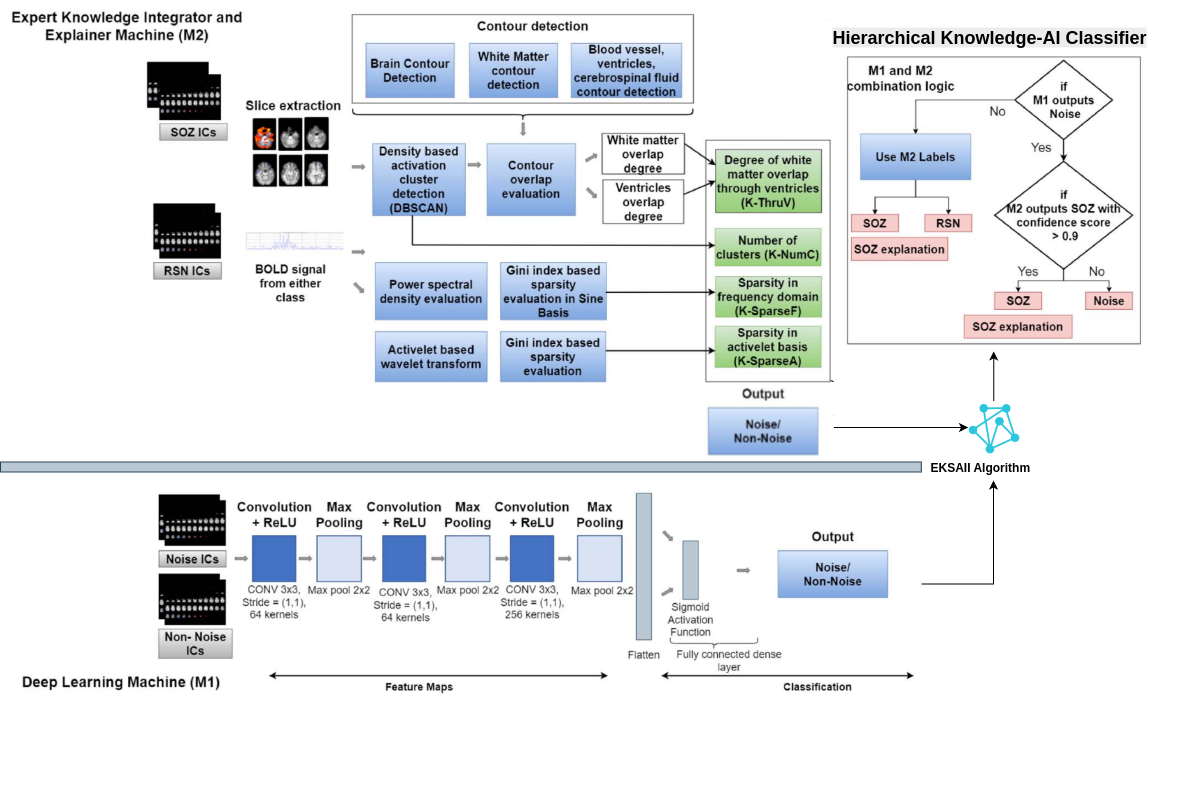
\includegraphics[width=0.8\columnwidth]{soz.png}
    \caption{
    \textbf{DeepXSOZ: A Hybrid Knowledge-AI Architecture for Seizure Onset Zone (SOZ) Localization.}
    The framework employs a bipartite training architecture. During inference, the final SOZ classification is determined by integrating the labels from both $\text{M}_{\text{DL}}$ and $\text{M}_{\text{CCKR}}$ via confidence scores, yielding a final, integrated, and explainable diagnostic result.
    }
    \label{fig:deepxsoz_framework}
\end{figure}

\begin{figure}[h!]
\scriptsize
    \centering
    \includegraphics[width=0.8\columnwidth]{dr.png}
    \caption{
    \textbf{Hierarchical Knowledge-AI Integration Framework for Diabetic Retinopathy (DR) Classification.}
    The system integrates a \textbf{Deep Learning Machine} ($M_d$, ViT backbone) and an \textbf{Expert Knowledge Machine} ($M_k$, clinical features/guidelines) within a decision tree.
    The \textbf{CCKR algorithm} iteratively selects the optimal binary classifier (maximum Entropy Imbalance Gain, EIG) for node splitting.
    }
    \label{fig:dr_framework}
\end{figure}
\begin{figure*}[ht]
    \centering
    % Reduce image width to make it smaller and neater
    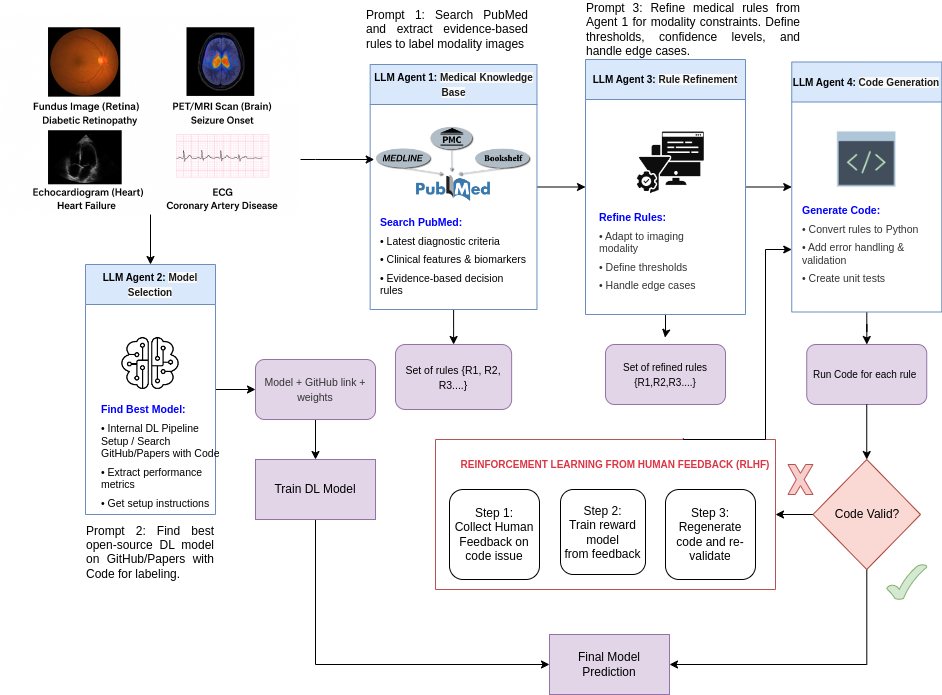
\includegraphics[width=0.75\textwidth]{main.png}
    \vspace{-2mm}
    \caption{\scriptsize\textbf{Agentic Knowledge-Guided Framework for Medical Image Labeling.} 
The proposed multi-agent system integrates medical knowledge retrieval, model selection, rule refinement, and code generation. 
\textbf{Agent 1} (CRA) searches PubMed and related sources to extract diagnostic rules and biomarkers per imaging modality.
\textbf{Agent 2} (CDA) identifies optimal open-source or (explicitly defined) DL models for labeling tasks.
CRA then refines rules from the expert medical knowledge extracted by Agent 1, adapting them to modality constraints and defining thresholds and confidence bounds.
\textbf{Agent 3} (CGA) converts refined rules into executable Python code, validated through an RLHF loop that corrects code errors using human feedback or relevant evaluation metrics. 
The final stage fuses knowledge-derived rules with DL predictions, enabling interpretable and generalizable medical image classification across modalities.}

    \label{fig:medxai_framework}
\end{figure*}

\end{document}
